\documentclass[12pt]{article}

% PACKAGES ---------------------------------------------------------------------
\usepackage[utf8]{inputenc}             % To write accents
\usepackage[english]{babel}             % So LaTeX do proper hyphenation
\usepackage[T1]{fontenc}                % Nicer default font (+ math font)
\usepackage{csquotes}                   % To use \enquote{}
\usepackage{titletoc}                   % Table of contents
                                        % -> must load before hyperref
\usepackage{hyperref}                   % Enable links
\usepackage[margin=1in]{geometry}       % To make pretty tables
\usepackage{booktabs}                   % To make pretty tables
\usepackage{tabularx}                   % To make pretty tables
\usepackage{mathtools}                  % Expand math tools
\usepackage{amsfonts}                   % Expand math tools
\usepackage{amsmath}                    % Expand math tools
\usepackage{amssymb}                    % Expand math tools
\usepackage{mathpazo}                   % Expand math tools
\usepackage{mathabx}                    % Expand math tools
\usepackage{graphicx}                   % Control figures
\usepackage[small,bf,center]{caption}   % Prettier figures
\usepackage{subfig}                     % Prettier figures
\usepackage{setspace}                   % ...
\usepackage{float}                      % To control figures' placement
\usepackage[section]{placeins}          % To control figures' placement
                                        % with \FloatBarrier
\usepackage{indentfirst}                % I like consistency!
\usepackage[toc,page]{appendix}         % To add appendices
\usepackage[authoryear]{natbib}         % References
  \bibliographystyle{chicago}           % -> style

% MATH SHORTCUTS ---------------------------------------------------------------

            % PENDING CLEAN UNUSED ONES !!!!!!!!!!!!!!!!!!!
\setcounter{secnumdepth}{0}
\let\IG\iffalse
\let\ENDIG\fi
\def\D{\displaystyle}
\def\td#1#2{\frac{\D \mathit{d} #1}{\D \mathit{d} #2}}
\def\std#1#2{\frac{\D \mathit{d}^2 #1}{\D \mathit{d} {#2}^2}}
\def\ctd#1#2#3{\frac{\D \mathit{d}^2 #1}{\D \mathit{d} #2 \mathit{d} #3}}
\def\pd#1#2{\frac{\D \partial #1}{\D \partial #2}}
\def\pdi#1#2{\partial #1/\partial #2}
\def\cpdi#1#2#3{\partial^2 #1/\partial #2 \partial #3}
\def\spdi#1#2{\partial^2 #1/\partial {#2}^2}
\def\spd#1#2{\frac{\D \partial^2 #1}{\D \partial {#2}^2}}
\def\cpd#1#2#3{\frac{\D \partial^2 #1}{\D \partial #2 \partial #3}}
\newcommand{\Lg}{\mathcal{L}}
\newcommand{\LR}{\Leftrightarrow}
\newcommand{\half}{\tfrac{1}{2}}
\newcommand{\qrtr}{\tfrac{1}{4}}
\newcommand{\eqs}{\buildrel s \over =}
\newcommand{\foc}[1]{\ensuremath{\text{foc}\mspace{2mu}#1}}
\newcommand{\cs}[1]{\ensuremath{\text{cs}\mspace{2mu}#1}}
\newcommand{\nn}[1]{\ensuremath{\text{nn}\mspace{2mu}#1}}
\allowdisplaybreaks

\newcommand{\brk}{\vspace*{0.8em}\hrule}


\newtheorem{prop}{Proposition}


\begin{document}


% FIRST PAGE -------------------------------------------------------------------


\title{\vspace{-3cm}
      Expecting to get it: \\ An endowment effect for information
      }

% ADD LINK TO UPTODATE VERSION AND SUPPLEMENTARY+REPLICATION MATERIAL

\author{Tabaré Capitán
          \thanks{Corresponding author: \href{mailto:Tabare.Capitan@gmail.com}{\texttt{Tabare.Capitan@gmail.com}}. For helpful comments or thoughtful discussions, we thank Hunt Allcott, Alec Brandon, James Heckman, Stephan Kroll, John List, Daniel Millinet, and Stephen Newbold. We also thank participants in seminars at UA Anchorage, the University of Chicago, Colorado State University, the 2019 North American Economic Science Association meetings, and the 2020 Bogotá Experimental Economics Conference. Financial support from USDA/NIFA (grant number 2016-09907) is gratefully acknowledged. The collection of data for this study was approved by the IRB at University of Wyoming.}
        \and
        Linda Thunström
        \and
        Klaas van ‘t Veld
          \\ \small{Department of Economics, University of Wyoming}
        \and
        Jonas Nordström
          \\ \small{Lund University and University of Copenhagen}
        }

\maketitle

\thispagestyle{empty}   % Suppress page number (must be under \maketitle)

\begin{abstract}

\noindent
We show, both theoretically and empirically, that an endowment effect for information arises from the expectation of getting information. Furthermore, we show that this endowment effect matters to welfare analysis of information policies, and can be put to advantage in situations where widespread dissemination of information is socially desirable (e.g., benefits of using masks during the COVID-19 global pandemic).
\\
\\
\textit{Keywords:} expectations, reference-dependent preferences, preferences for information, information avoidance.
\\
\textit{JEL classification:} D01, D80, D83, D84, D91, C91.

\end{abstract}

\clearpage

\pagenumbering{arabic} % Start numbering in page 2 from #1



% PAPER ------------------------------------------------------------------------

\section{Introduction}

  % CONCRETE EXAMPLE -------------------------------------------------------------

Ana and Beto, separately, have decided to go to a café to eat a chocolate cake. Both are equally concerned about their calorie intake and have the same belief about the calorie content of the cake, but Ana expects the café to have calorie information on the menu and Beto does not. In this paper we show, both theoretically and empirically, that Ana’s expectation makes the information more valuable to her than to Beto.  In other words, an endowment effect for information arises from the very expectation of getting the information. We are not aware of previous work in which this endowment effect has been identified, let alone tested.\footnote{However, at least two previous studies provide suggestive evidence of an endowment effect for information. First,  \citet{cawleyImpactInformationDisclosure2020} find that participants with high exposure to calorie information are more supportive of calorie labels. Second, \cite{nordstromStrategicIgnoranceHealth2020} find that participants that have been informed about the calorie content in a meal are more likely to state that they would have used the calorie information, compared to participants that could choose to be informed or not.}

% INFORMATION VS RISK ----------------------------------------------------------

% COMMENTS

% KLAAS:  the parenthetical bits in (third sentence) read *too* terse to me now. The reader won’t understand the mapping from risk to information, and you don’t want to lose her 1.5 paragraphs into the paper.
% -> Expanded "a non-degenerate lottery defined by a prior distribution of beliefs ABOUT THE INFORMATION"


The endowment effect we observe is closely related to the endowment effect for risk predicted by the theory of \citet{koszegiReferenceDependentRiskAttitudes2007} and tested by \citet{sprengerEndowmentEffectRisk2015}. Their endowment effect for risk arises because those expecting to face risk (a non-degenerate lottery over consumption outcomes) are more tolerant to risk than those expecting to face an outcome that is certain. In our case, expecting to receive information is akin to expecting to face risk (a non-degenerate lottery defined by a prior distribution of beliefs about the information), whereas \emph{not} expecting to receive information is akin to expecting an outcome that is certain (the mathematical expectation of the prior distribution of beliefs about the information).\footnote{\citet{koszegiReferenceDependentConsumptionPlans2009} develop another theory of expectations-based reference-dependent preferences\textemdash\emph{news utility}\textemdash that might seem closer to our work. However, this theory is about reference-dependence with respect to the \emph{content} of the information (i.e., what you might find out). Instead, the endowment effect for information arises from reference-dependence with respect to information \emph{delivery} (i.e., whether you find out), regardless of the content.}

% PONDERING WHAT'S BEST TO START THIS PARAGRAPH:
% Yet the parallel to an endowment effect for risk is not perfect.
% But the parallel to an endowment effect for risk is not perfect.
% However, the parallel to an endowment effect for risk is not perfect.
% The parallel to an endowment effect for risk is not perfect, however. (Klaas)
% Even so, the parallel to an endowment effect for risk is not perfect.

However, the parallel to an endowment effect for risk is not perfect. Because the role of information in decision making goes beyond mere updating of beliefs, preferences for risk are not the same as preferences for information. Instrumental information can be used to adjust behavior (e.g., calorie information can induce Ana or Beto to eat less or more of their cake, or exercise more or less strenuously afterwards), and even non-instrumental information can simply spark curiosity \citep{loewensteinPsychologyCuriosityReview1994,sharotHowPeopleDecide2020}.

% THEORY -----------------------------------------------------------------------

Our endowment effect for information fits in the theoretical literature on expectations-based reference-dependent preferences \citep{marzilliericsonEndowmentEffect2014,odonoghueChapterReferenceDependentPreferences2018}.\footnote{\citet{sprengerEndowmentEffectRisk2015} reviews the related empirical literature, concluding that \enquote{Though both positive and negative results have been documented, an account of the literature would indicate some promise for the relevance of expectations in rationalizing reference-dependent behavior} (p1458).} In this literature, utility is separated into intrinsic utility (i.e., utility from outcomes) and gain-loss utility (i.e., utility from comparing outcomes to a referent). While the intrinsic utility is typically modeled in the same way across different theories, the specification of the gain-loss utility differs between the two leading theoretical approaches. The Disappointment Aversion approach \citep{bellDisappointmentDecisionMaking1985,loomesDisappointmentDynamicConsistency1986,gulTheoryDisappointmentAversion1991} collapses the reference lottery into a single value and measures the gain-loss utility relative to that value. In contrast, the  Kőszegi and Rabin approach \citep{koszegiModelReferenceDependentPreferences2006,koszegiReferenceDependentRiskAttitudes2007} measures the gain-loss utility from every element of the outcome lottery relative to each element of the reference lottery separately, and then aggregates these gain-loss utilities to a single value.\footnote{Consequently, the distinction between these two theoretical approaches is consequential only when the referent is stochastic, i.e., a reference lottery.}  In this paper, we show that both approaches predict an endowment effect for instrumental information, but only the Kőszegi and Rabin approach predicts an endowment effect for non-instrumental information.

% EXPERIMENTAL EVIDENCE --------------------------------------------------------

In addition, we find evidence consistent with an endowment effect for information in a two-stage laboratory experiment, in which we offer participants a free cake and manipulate their expectations about whether they will get information about the cake’s calorie content. The idea of manipulating expectations to investigate the endowment effect builds on \possessivecitet{koszegiModelReferenceDependentPreferences2006} definition of a person’s referent as not the status quo, but rather \enquote{the \emph{expectations} a person held in the \emph{recent} past}, or more specifically \enquote{her probabilistic beliefs about the relevant consumption outcome held between the time she first focused on the decision determining the outcome and shortly before consumption occurs} (p.1141). Hence, the status quo can be viewed as a special case of this more general definition: in most experiments that treat the status quo as the referent, subjects plausibly expect the status quo to continue in the future.

In the first stage, we vary participants’ \emph{experience} with calorie information to vary their sense of endowment. All participants are asked to choose their preferred dessert from eleven consecutive different menus, but those menus show calorie information for only half of the participants, and no calorie information for the other half. This priming manipulation is motivated by \possessivecitet{koszegiModelReferenceDependentPreferences2006} rationalization of \possessivecitet{listDoesMarketExperience2003} empirical finding that market experience reduces the (standard) endowment effect. The argument is that, because experienced traders are more likely to expect to trade their acquisitions, the endowment effect for them is smaller. More specifically, because experienced traders are less likely to extrapolate the status quo of having owned an item in the recent past to an expectation of retaining the item in the future, they experience less loss aversion when parting with the item through trading it away. As a result, they behave more like they would if they never owned the item in the first place, and in that sense exhibit less of an endowment effect.\footnote{List shows that market experience reduces the endowment effect in two related papers \citep{listDoesMarketExperience2003, listDoesMarketExperience2011}.
The key issue to identify the effect of market experience on the endowment effect is that market experience is endogenous (i.e., experienced traders might be experienced precisely because of their lower endowment effect). In his first paper \cite{listDoesMarketExperience2003} \enquote{attempts to econometrically parse treatment (market experience) from selection, (but) his results rely on his modeling assumptions} (p.314), and in his second paper \cite{listDoesMarketExperience2011} \enquote{attempts to rectify this issue (i.e., relying on modeling assumptions) by making market experience exogenous} (p. 314). Although \citet{koszegiModelReferenceDependentPreferences2006} rationalize the empirical finding as presented in the first paper \citep{listDoesMarketExperience2003}, our experimental design is closer to \citep{listDoesMarketExperience2011} because we also use a two-stage experiment in which first manipulate experience (using menus with calorie information) and then manipulate the endowment (or expectation to receive information). Hence, we are able to identify the endowment effect for information separately for unexperienced and experienced participants, without relying on modeling assumptions.}

% unexperience: 51% -> 70%
% experience:   60% -> 65%

Our manipulation applies the argument in the opposite direction. Whereas List’s experienced traders already expected to \emph{give up} items in their transaction, through their frequent exposure to trading, our experienced participants (in the second stage) should already expect to \emph{gain} information, through their frequent exposure to seeing it on menus (in the first stage). Experienced participants, we therefore predict, should be less likely to extrapolate the status quo of \emph{not} having information to an expectation of not getting it in future, and thus experience \emph{more} loss aversion when giving up the information (i.e., their referent is more likely to be getting the information). As a result, they will behave more like they would if they felt endowed with the information in the first place, and in that sense exhibit less of an endowment effect.\footnote{Note that the endowment \enquote{effect} is defined as a difference in behavior (e.g., willingness to trade a mug for a pen) depending on one’s sense of endowment. List’s experienced traders behaved similarly whether or not they were endowed with an item, thus exhibiting no endowment effect. We predict that experienced participants will also behave similarly whether or not they are endowed with information, thus again exhibiting no endowment effect.}

In the second stage, we vary participants' \emph{first-focus} on calorie information to vary their sense of endowment. All participants are asked if they want to learn the calorie content of three desserts on a menu, one of which, a cake, is marked as theirs to receive. For half of the participants, the menu includes a calorie-information column with the actual calorie numbers \enquote{temporarily} \emph{xxx}-ed out; for the other half, the menu shows nothing calorie-related. This is the key manipulation of our experiment. It builds on the first-focus intuition implied by \possessivecitet{koszegiModelReferenceDependentPreferences2006} definition of the referent, which \citet{sprengerEndowmentEffectRisk2015} also exploits to test the endowment effect for risk.\footnote{Sprenger notes that the intuition is \enquote{in line with the psychological literature on \enquote{cognitive reference points} (Rosch 1974) and decision anchoring} (p.1462), which has shown referents to be susceptible to experimental variation.} Specifically, the \emph{xxx}-ed out calorie column on the first group's menu is intended to make participants focus first on getting calorie information when considering their choice whether to actually see it, and in that sense feel \emph{endowed} with the information. Conversely, the absence of any calorie-related information on the second group's menu is intended to make participants focus first on not getting information when considering the same choice, and in that sense feel \emph{not endowed} with the information.\footnote{Although we label our participants as \emph{endowed} or \emph{not endowed}, we do not claim that our manipulation \emph{fully} sets the referent. Instead, our experimental manipulations vary the \emph{degree} to which participants feel endowed with the information. A more precise way to label our participants, used by \citet{heffetzEndowmentEffectExpectations2014}, would be to use \emph{more endowed} and \emph{less endowed}. Nevertheless, we favor our labels to be consistent with the language typically used in the literature on the endowment effect.}

Our results support the existence of an endowment effect for information, in line with our theoretical prediction: among participants not primed in the first stage to expect calorie information, those endowed with information in the second stage asked to keep the information significantly more often than non-endowed participants asked to add it. Moreover, consistent with the argument that experience with information matters, this endowment effect was much weaker, and not statistically significant, for participants primed in the first stage to expect information.

% POLICY IMPLICATIONS ----------------------------------------------------------

This endowment effect has implications for welfare analysis of policies that mandate, encourage, or restrict, the delivery of various kinds of information. Examples include the Right-to-Know acts and eco-label programs (e.g., USDA organic and Energy Star) in environmental regulation; GMO, nutritional, and calorie labeling in agricultural and food regulation; graphic warnings on cigarette packaging, disclosure of medical risks and side effects, and diagnostic testing in health regulation; SEC financial disclosure (e.g., Sarbanes-Oxley) and mortgage disclosure in financial regulation; and ethical labels (e.g., animal cruelty and child labor), financial disclosure by politicians, and conflict-mineral content in other areas. These information policies are ubiquitous and often subject to cost-benefit analysis (CBA) requirements.

Under the traditional assumption (in economics) that the value of information is always non-negative \citep{stiglerEconomicsInformation1961}, CBA is straightforward in principle: the only hurdle that needs to be checked is that estimated information benefits outweigh (often low) implementation costs. But recent research (reviewed by \citet{golmanInformationAvoidance2017}) has challenged the traditional assumption, noting that information can evoke negative feelings such as anxiety or guilt, so that even costless information can harm people (i.e., the value of information can be negative).\footnote{For example, if information evokes negative emotions or feelings (e.g., anxiety, fear, guilt, regret, annoyance, or pain), these negative emotions or feelings might lead to information avoidance \citep{koszegiHealthAnxietyPatient2003,danaExploitingMoralWiggle2007,karlssonOstrichEffectSelective2009,sweenyInformationAvoidanceWho2010,osterOptimalExpectationsLimited2013,grossmanStrategicIgnoranceRobustness2014,hertwigHomoIgnoransDeliberately2016,onwezenWhenIndifferenceAmbivalence2016,savolainenApproachingAffectiveBarriers2016,thunstromStrategicSelfignorance2016,grossmanSelfImageWillfulIgnorance2017,damgaardHiddenCostsNudging2018,thunstromEndogenousAttentionCosts2019,sunsteinRuiningPopcornWelfare2019}.} The possibility to do harm with information policies complicates welfare analysis because\textemdash even ignoring the cost of implementation\textemdash their welfare effects can range from negative to positive \citep{damgaardHiddenCostsNudging2018, allcottWelfareEffectsNudges2019,buteraDeadweightLossSocial2019,rafiqHowMuchCalorieundefined/ed,thunstromWelfareEffectsNudges2020}.\footnote{The complication is greater if there is heterogeneity in negative feelings \citep{sunsteinRuiningPopcornWelfare2019}, or in the ability to respond to information \citep{robertsNudgeProofDistributiveJustice2018}}

Our findings point to further complications. Most immediately, the existence of an endowment effect for information implies that the outcome of welfare analysis may depend on timing. Consider, for example, a cost-benefit analysis of a policy that requires cafés to provide calorie information on their menus. In the presence of experience effects like those identified in our experiment, this analysis would be more likely to conclude in favor of the policy if conducted after the policy’s introduction, when people have come to expect the information. More generally, the existence of an endowment effect for information implies that the role of the referent, including potential heterogeneity of referents across consumers, ought to be explicitly acknowledged and accounted for in welfare analysis.

     % XXXXXXXX    PARAGRAPH BELOW NEEDS SOME WORK     XXXXXXXXXXXXXX %

On the positive side, the endowment effect for information may provide a new policy tool to reduce avoidance of \enquote{good} information, such as information about health and financial risks. The goal of this policy tool would be to raise people's expectation to receive information and, via the endowment effect, thereby increase their valuation of that information (leading to less information avoidance). For example, during the COVID-19 pandemic, people might be less likely to ignore information about the risks of engaging in various activities if they expect to get such information.

We return to the discussion of welfare implications in the concluding section, after first introducing our theoretical framework and empirical evidence in the next sections.


\section{Theory: Disappointment Aversion and the \\ Kőszegi and Rabin approach}

  We model information preferences\textemdash preferences for taking or avoiding information\textemdash by applying and extending two theoretical approaches to modeling expectations-based reference-dependent preferences. One is the Disappointment Aversion (hereafter DA) approach pioneered by \citet{bellDisappointmentDecisionMaking1985}, with later contributions by \citet{loomesDisappointmentDynamicConsistency1986} and \citet{gulTheoryDisappointmentAversion1991}; the other is the Kőszegi and Rabin (hereafter KR) approach developed by Kőszegi and Rabin \citep{koszegiModelReferenceDependentPreferences2006,koszegiReferenceDependentRiskAttitudes2007}. In our exposition, we follow the notation of \citet{odonoghueChapterReferenceDependentPreferences2018} to discuss both approaches in a unified framework.

Formally, both approaches define the utility from a lottery of outcomes $L \equiv (x_1,p_1;x_2,p_2;...;x_N,p_N)$ given a reference lottery $R \equiv (r_1,q_1;r_2,q_2;...;r_M,q_M)$ as
\begin{equation*}
  U(L|R) \equiv \sum_{n=1}^{N} p_n[u(x_n)+v(x_n|R)],
\end{equation*}
where $u(x_n)$ is the intrinsic utility from lottery outcome $x_n$ and $v(x_n|R)$ is the gain-loss utility associated with that outcome. That is, $U(L|R)$ is the expected sum of intrinsic and gain-loss utility from each outcome of $L$.

The DA approach specifies the gain-loss utility from a specific outcome $x_n$ (from the lottery $L$) as
\begin{equation*}
  v(x_n|R) \equiv \mu (u(x_n)-\sum_{m=1}^M q_mu(r_m)),
\end{equation*}
i.e., as involving a comparison of the intrinsic utility of $x_n$ to the expected intrinsic utility from the reference lottery $R$. The gain-loss utility function $\mu(\cdot)$ is thereby specified as the piece-wise linear function
\begin{equation*}
  \mu(z)=
  \begin{cases}
    z          & \text{if } z \geq 0 \\
    \lambda z  & \text{if } z < 0 ,
  \end{cases}
\end{equation*}
where $\lambda>1$ (implying loss aversion). That is, if $u(x_n)$ is greater than $E[u(r_m)]$, this gives rise to gain utility $u(x_n)-E[u(r_m)]$, but if $u(x_n)$ is less than $E[u(r_m)]$, it gives rise to larger (in absolute terms) loss utility $\lambda(u(x_n)-E[u(r_m)])$.

In contrast, the KR approach specifies
\begin{equation*}
  v(x_n|R) \equiv \sum_{m=1}^M q_m \mu (u(x_n)-u(r_m));
\end{equation*}
that is, each outcome $x_n$ (from lottery $L$) is compared \emph{separately} to each individual outcome $r_m$ of the reference lottery $R$, giving rise (again with the same piece-wise linear gain-loss utility function) to gain utility $u(x_n)-u(r_m)$ if $u(x_n) \geq u(r_m)$ and to loss utility $\lambda [u(x_n)-u(r_m)]$ if $u(x_n)<u(r_m)$. The overall gain-loss utility $v(x_n|R)$ is the sum of all those separate gain and loss utility components, weighted by the probability $q_m$ of each outcome in $R$ that $x_n$ is compared to.

To make things more concrete and discuss the model in the context of preferences for information, consider our two cake eaters, Ana and Beto.\footnote{We emphasize that, in our example, Ana (who expects to receive information) and Beto (who expects not to receive information) are essentially the same person, except for their differing expectations.} Ana and Beto know that it is equally probable that the cake they are about to eat is either low- or high-calorie, and because they are both equally concerned about their calorie intake, their intrinsic utility of eating a high-calorie cake is \emph{low} ($\ell$), and their intrinsic utility of eating a low-calorie cake is \emph{high} ($h$). Furthermore, they do not anticipate being able to tell the cake’s calorie content from eating it, and, for now, they do not anticipate adjusting their behavior in response to the calorie information (i.e., the information is non-instrumental). Therefore, if they do not receive information about the calorie content of the cake, they will perceive eating the cake as yielding intrinsic utility $\half h + \half \ell$ (i.e., the probability weighted average of their utility in the low- and high-calorie states of the world).

Written in terms of lotteries, and for simplicity equating lottery outcomes with their induced utilities (i.e., skipping the intermediate step of mapping calories to intrinsic utilities), we can represent their situation if they currently do not know the cake's calorie content but will find out, as facing the lottery $L^i$ (superscript $i$ for \emph{informed}) equal to $(x_1=h,p=\half;x_2=\ell,p_2=\half)$. If they will \emph{not} find out, however, then they face the degenerate lottery $L^u$ (superscript $u$ for \emph{uninformed}) equal to $(x=\half h + \half \ell,p=1)$.

If their utility is reference-dependent, then their evaluation of these lotteries will depend on whether they \emph{expect} to be informed (i.e., see calorie information in the menu). For Ana, who expects to be informed, we can represent this as starting out with reference lottery $R^i=(r_1=h,q_1=\half;r_2=\ell,q_2=\half)$; for Beto, who expects not to be informed, we can represent this as starting with degenerate reference lottery $R^u=(r=\half h + \half \ell,q=1)$. Thus, there are four possible utilities:
\begin{itemize}
	\item $U(L^i|R^i)$ from expecting to be informed and getting information,
	\item $U(L^u|R^i)$ from expecting to be informed and not getting information,
	\item $U(L^i|R^u)$ from expecting to be uninformed and getting information, and
  \item $U(L^u|R^u)$ from expecting to be uninformed and not getting information.
\end{itemize}

An endowment effect is predicted if receiving the information is more valuable to a person who expects to receive it (like Ana) than to a person who does not expect to receive it (like Beto):\footnote{\citet{sprengerEndowmentEffectRisk2015} emphasizes that the KR endowment effect for risk that he tests for \enquote{should be thought of as distinct from the standard endowment effect literature documenting exchange anomalies as discrepancies between WTP and WTA for the same object. The KR endowment effect for risk is a risk preference discrepancy between risk taking when the referent is certain and risk taking when the referent is stochastic.} (p.1458) Similarly, in our context, the endowment effect for information is an information preference discrepancy between information seeking when the referent is certain (i.e., an agent does not expect to receive information, making the referent a degenerate lottery) and information seeking when the referent is stochastic (i.e., the agent expects to receive information, making the referent a non-degenerate lottery).}
\begin{equation}
  U(L^i|R^i)-U(L^u|R^i)>U(L^i|R^u)-U(L^u|R^u).
  \label{eq:endowmentEffect}
\end{equation}

Below we discuss four results regarding the existence of an endowment effect for information under the DA or the KR approach when information is either non-instrumental or instrumental. See Appendix \ref{appendix:theory} for all derivations the derivations.

\begin{prop}
  Assume reference-dependent utility following the DA approach, with a piece-wise linear gain-loss utility function and non-instrumental information. For any lottery $L$, $U(L^i|R^i)-U(L^u|R^i)=U(L^i|R^u)-U(L^u|R^u)$. Therefore, no endowment effect is predicted.
  \label{prop:nonInstrumental-DA}
\end{prop}

\begin{figure}[ht]
  \caption{Value of information under the DA approach, with non-instrumental information.}\label{fig:nonInstrumental-DA}
  \begin{center}
  {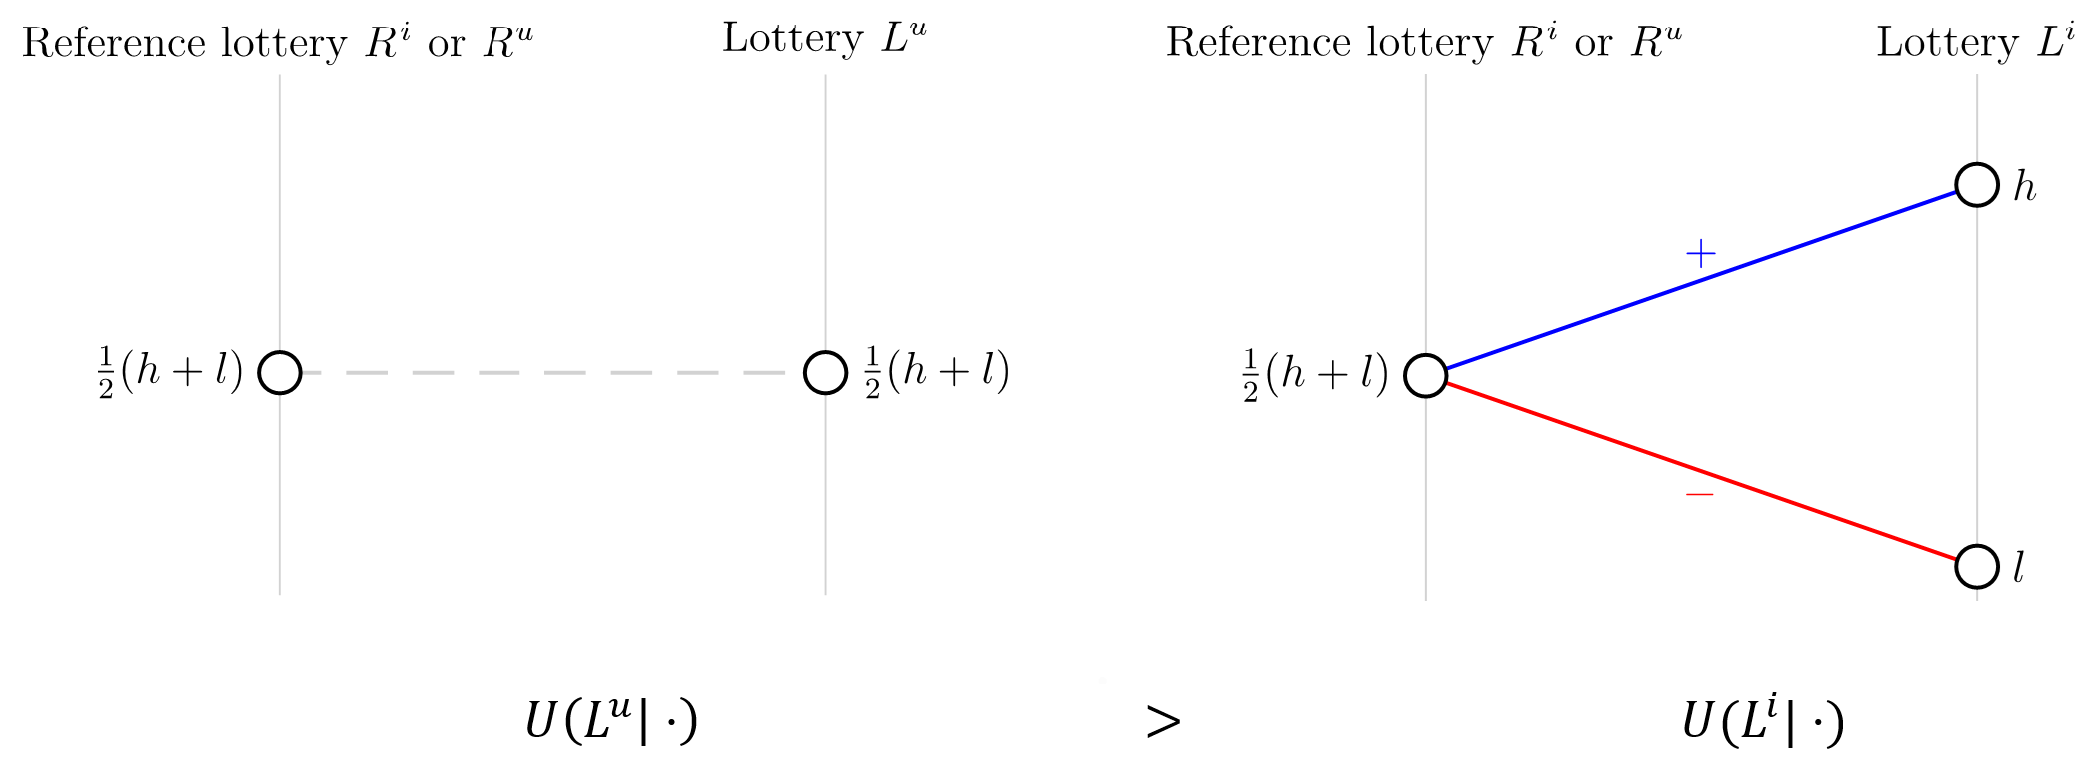
\includegraphics[width=1\textwidth]{./figures/theory_fig1.png}}
  \end{center}
\end{figure}

Because under the DA approach the reference lottery collapses to its expectation before evaluating gain-loss utility, and given that both referents $R^i$ and $R^u$ have the same expectation $E[R^i]=E[R^u]=\half(h+\ell)$, the difference $U(L^i|\cdot)-U(L^u|\cdot)$ is the same regardless of whether a person expects to receive information or not. Specifically, as illustrated in Figure \ref{fig:nonInstrumental-DA}, relative to not getting information (illustrated in the left panel), getting information (illustrated in the right panel) involves a gain of $h-\half(h+\ell)=\half(h-\ell)$ with probability one-half and a utility loss of $l-\half(h+\ell)=-\half(h-\ell)$ with probability one-half. Because of loss aversion, however, the utility loss receives additional weight $\lambda>1$, implying that $U(L^i|\cdot)-U(L^u|\cdot)=-\qrtr(\lambda-1)(h-\ell)<0$. In other words, the value of information is equally negative, regardless of expectations.

\FloatBarrier

\begin{prop}
  Assume reference-dependent utility following the KR approach, with a piece-wise linear gain-loss utility function and non-instrumental information. For any lottery $L$, $U(L^i|R^i)-U(L^u|R^i)>(L^i|R^u)-U(L^u|R^u)$. Therefore, an endowment effect is predicted.
  \label{prop:nonInstrumental-KR}
\end{prop}

\begin{figure}[ht]
  \caption{Value of information under the KR approach, with non-instrumental information.}\label{fig:nonInstrumental-KR}
  \begin{center}
  {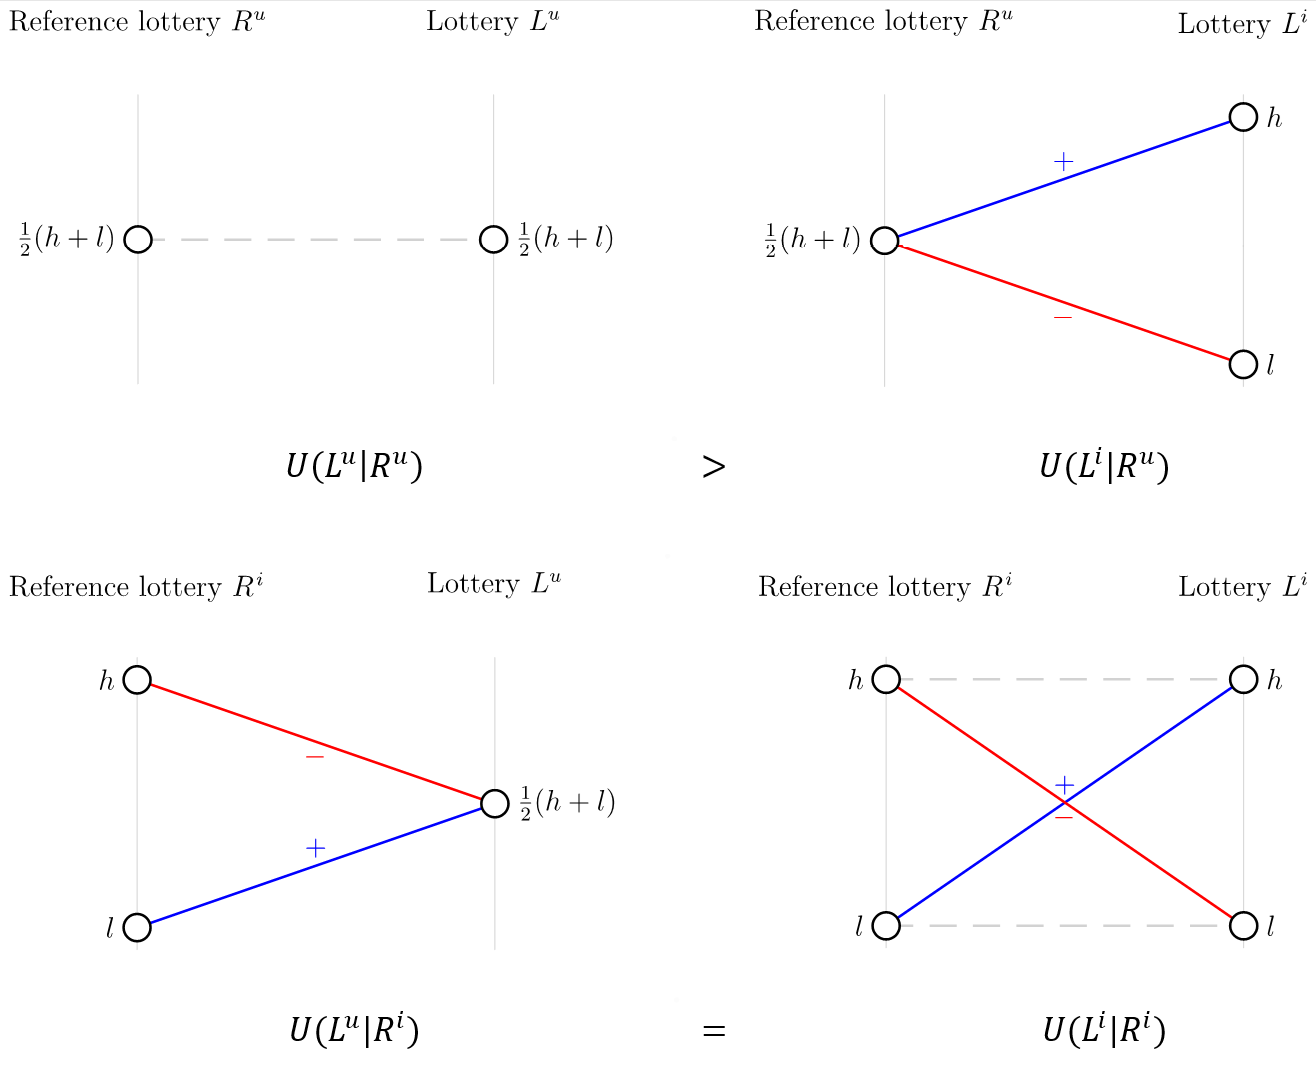
\includegraphics[width=1\textwidth]{./figures/theory_fig2.png}}
  \end{center}
\end{figure}

Figure \ref{fig:nonInstrumental-KR} illustrates how the endowment effect for information arises under the KR approach. Since all four possible outcomes yield the same intrinsic utility $\half(h+\ell)$, the endowment effect is driven by differences in gain-loss utility depending on expectations.

If information is not expected (illustrated in the top panels), getting it results in the same net utility loss $U(L^i|R^u)-U(L^u|R^u)=-\qrtr(\lambda-1)(h-\ell)<0$ as under the DA approach. In other words, Beto's value of information is negative\textemdash{he is information averse}.

If information is expected (illustrated in the bottom panels), then not getting it (the bottom-left panel) involves a utility gain of $\half(h+\ell)-\ell=\half(h-\ell)$ and a loss $\half(h+\ell)-h=-\half(h-\ell)$, each weighted by probability one-half. Because the loss receives additional weight $\lambda>1$, the net gain-loss utility is $-\qrtr(\lambda-1)(h-\ell)<0$. But\textemdash and this is key\textemdash getting information that is expected (the bottom-right panel) involves a \emph{twice larger} utility gain of $(h-\ell)$ and loss of $-(h-\ell)$, each weighted \emph{twice smaller} probability one-quarter, before applying outcomes $\ell$ in both. On net, then, the gain-loss utility ends up being the same $-\qrtr(\lambda-1)(h-\ell)<0$, implying that $U(L^i|R^i)-U(L^u|R^i)=0$. In other words, Ana's value of information is zero\textemdash{she is information neutral}.

Comparing Ana's and Beto's value of information, we find an endowment effect:
\begin{equation*}
  [U(L^i|R^i)-U(L^u|R^i)]-[U(L^i|R^u)-U(L^u|R^u)]=\qrtr(\lambda-1)(h-\ell)>0.
\end{equation*}
Note that, at least for non-instrumental information, the endowment effect does not make Ana value information more positively. Rather, it makes her value information \emph{less negatively}: she becomes information neutral rather than information averse.

Proposition \ref{prop:nonInstrumental-KR} is closely related to the prediction of an endowment effect for risk in \citet{koszegiReferenceDependentRiskAttitudes2007}. In fact, we have treated information in a way that parallels the way monetary risk is treated in their model: expecting to receive information is akin to having a stochastic referent, and expecting not to receive information is akin to having a non-stochastic referent.

The parallel extends further than Kőszegi and Rabin’s characterization of the psychology underlying their endowment effect for risk. They remark that their predictions crucially \enquote{do \emph{not} imply that a person is unbothered by risk she expects or faces, even if it does make her less risk averse.} Rather, a decisionmaker who had been expecting risk, or is already facing risk, \enquote{is already exposed to stochastic utility-decreasing sensations of loss, so taking additional risk does not add so much exposure to losses} (p. 1054). In our context, the endowment effect for information may arise similarly because those who expect information have already built utility-decreasing sensations of loss into their expected utility. In other words, those who expect information are more willing to get it, because they are already exposed to the potential pain of disappointment outweighing the potential joy of pleasant surprise.

\FloatBarrier

Up until this point, we have assumed that information is non-instrumental. Because of this, information has served a role only in determining whether a lottery is degenerate or not, making our application so far indistinguishable from applications analyzing monetary risk. However, information can serve the additional role of allowing people to adjust current and future choices in response to it. For example, if Ana or Beto learn the calorie content of the cake, they can decide to eat less or more of  it, or adjust how much they subsequently exercise.

Suppose for simplicity that these adjustments would increase their utility by the same amount $\Delta > 0$ in both states of the world, and define $h^* \equiv h+\Delta$ and $\ell^* \equiv \ell+\Delta$. Thus, given her expectation of learning the calorie content of the cake, Ana expects to be able to make adjustments and get intrinsic utility $\half(h^*+\ell^*)$. Assuming adjustments are not so large to turn bad news into good news, which requires $\Delta <\half(h-l)$, we then have propositions \ref{prop:instrumental-DA} and \ref{prop:instrumental-KR}.

\begin{prop}
  Assume reference-dependent utility following the DA approach, with a piece-wise linear gain-loss utility function and instrumental information. For any lottery $L$, $U(L^i|R^i)-U(L^u|R^i)>(L^i|R^u)-U(L^u|R^u)$. Therefore, an endowment effect is predicted.
  \label{prop:instrumental-DA}
\end{prop}

\begin{figure}[ht]
  \caption{Value of information under the DA approach, with instrumental information.}\label{fig:instrumental-DA}
  \begin{center}
  {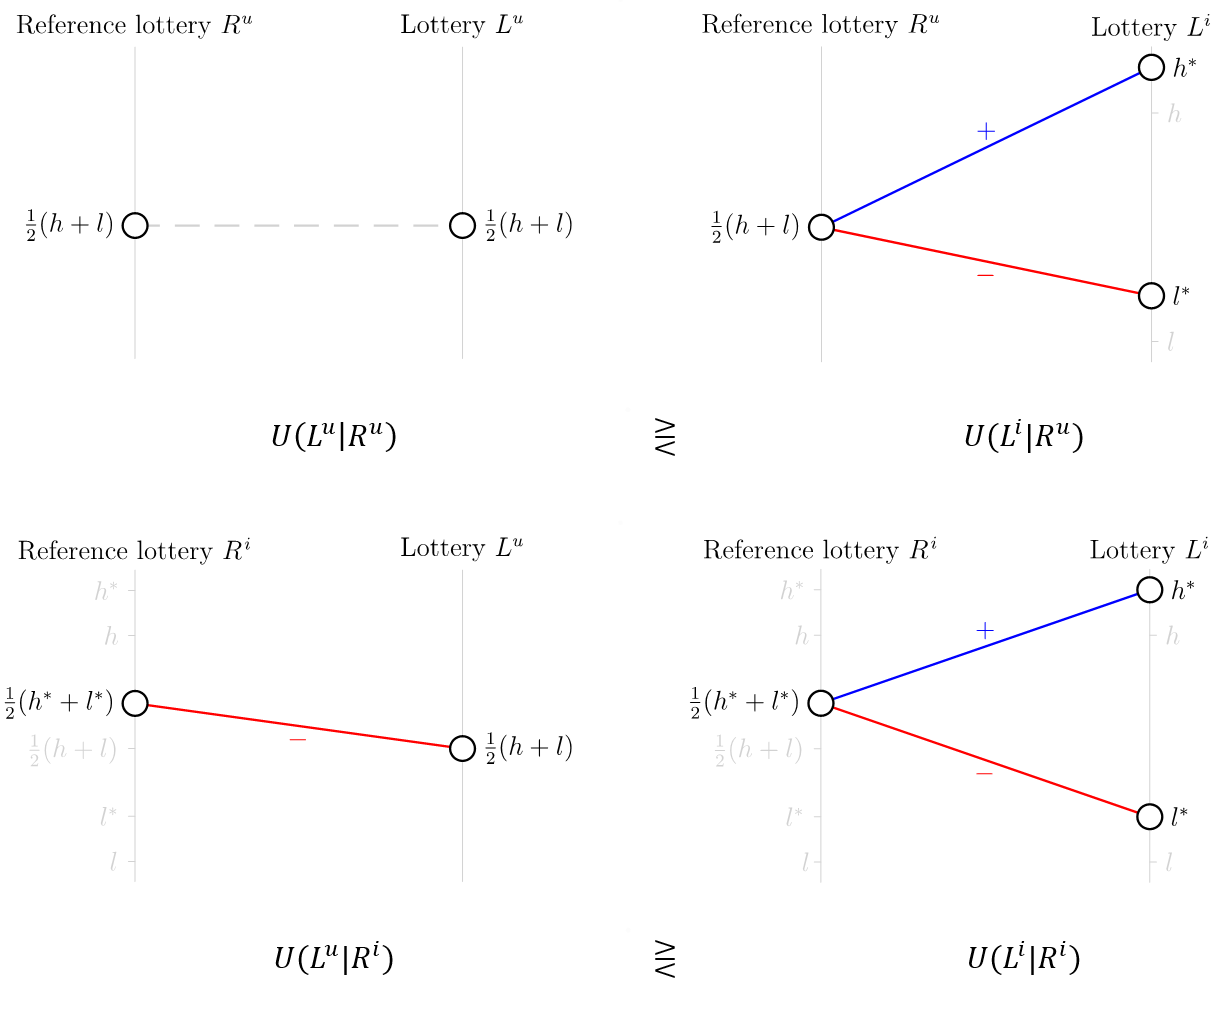
\includegraphics[width=1\textwidth]{./figures/theory_fig3.png}}
  \end{center}
\end{figure}

Figure \ref{fig:instrumental-DA} illustrates how the endowment effect now arises under the DA approach as well. The ability to make behavioral adjustments adds $\half \Delta + \half \Delta = \Delta$ to the intrinsic utility of getting information, regardless of expectations. If information is unexpected (illustrated in the top panels), however, then the gained ability to adjust enhances the gain from the good outcome and mitigates the loss from the bad outcome, thereby adding $\half \Delta + \half \lambda \Delta = \half (1 + \lambda) \Delta$ to gain-loss utility. The overall value of unexpected information becomes
\begin{equation*}
  U(L^i|R^u)-U(L^u|R^u)=-\qrtr(\lambda-1)(h-\ell)+\Delta +\half(1+\lambda)\Delta,
\end{equation*}
which for large enough $\Delta$ may be positive.

If information is expected (illustrated in the botoom panels), then the \emph{forgone} ability to adjust gives rise to loss utility $-\half \Delta - \half \lambda \Delta = -\lambda \Delta$ from \emph{not} getting information (the bottom-left panel). Because both the $R^i$ and $L^i$ lotteries shift up by the same amount $\Delta$, however, gain-loss utility from getting information (the bottom-right panel) is unchanged. The overall value of expected information therefore becomes
\begin{equation*}
  U(L^i|R^i)-U(L^u|R^i)=-0.25(\lambda-1)(h-l)+\lambda +\lambda \Delta
\end{equation*}

Moreover, because $\lambda>1$ implies that $\lambda \Delta > \half(1+\lambda)\Delta$, the value of expected information now exceeds that of unexpected information, implying an endowment effect. In short, the ability to adjust enhances the value of expected information by an avoided sure loss of $\lambda \Delta$, but the value of unexpected information by an avoided loss of $\lambda \Delta$ only with probability one-half, together with a gain of $\Delta$ with probability one-half. If losses outweigh gains, the former effect dominates.

\FloatBarrier

\begin{prop}
  Assume reference-dependent utility following the KR approach, with a piece-wise linear gain-loss utility function and instrumental information. For any lottery $L$, $U(L^i|R^i)-U(L^u|R^i)>(L^i|R^u)-U(L^u|R^u)$. Therefore, an endowment effect is predicted.
  \label{prop:instrumental-KR}
\end{prop}

\begin{figure}[ht]
  \caption{Value of information under the DA approach, with instrumental information.}\label{fig:instrumental-KR}
  \begin{center}
  {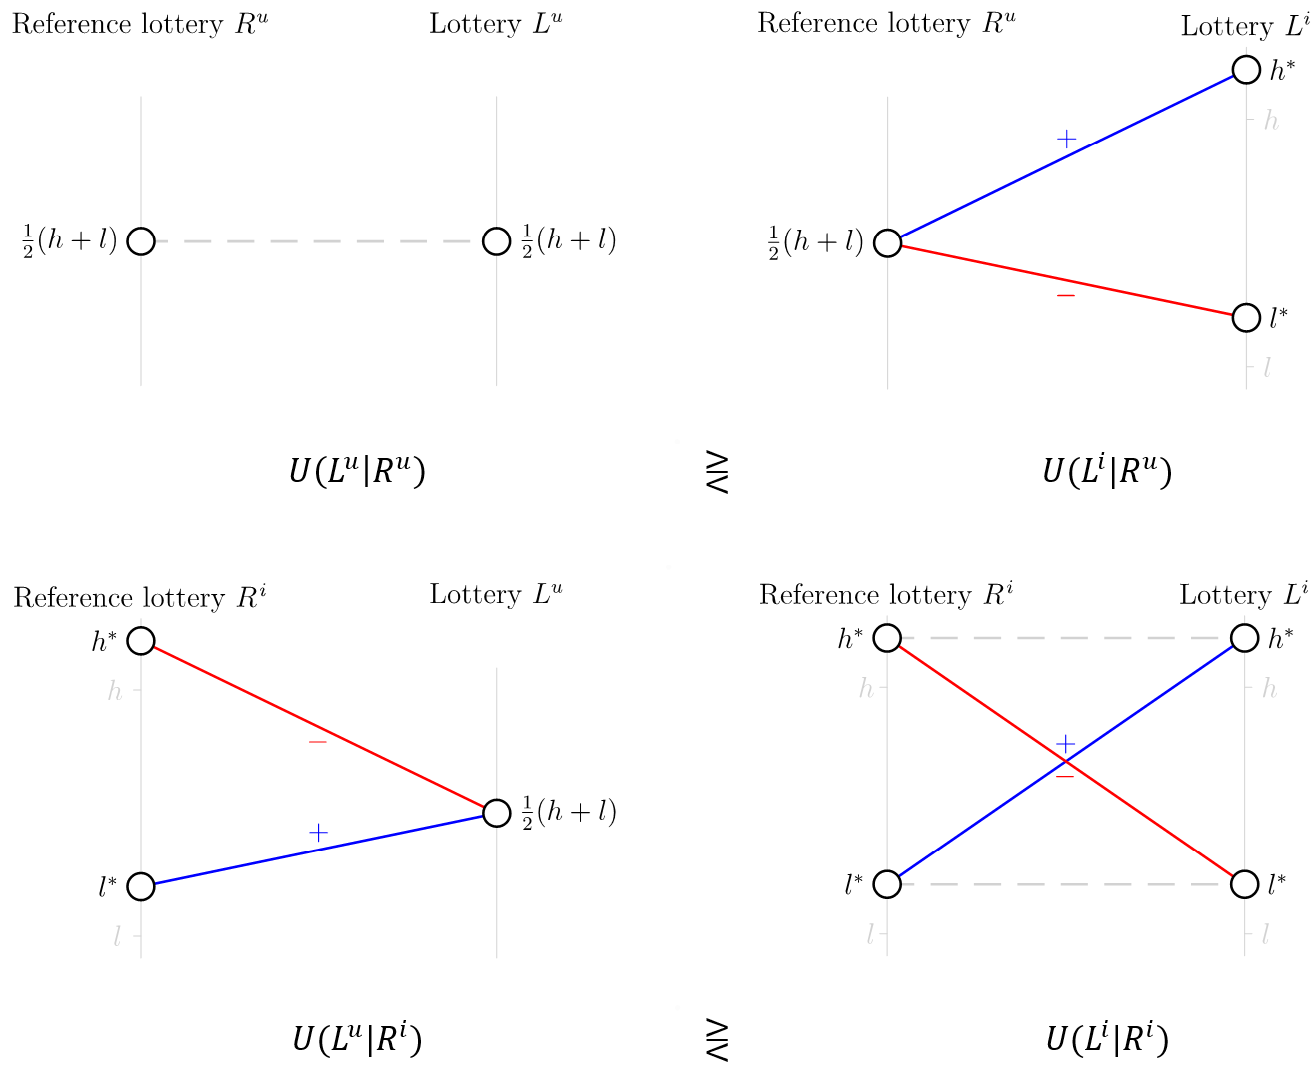
\includegraphics[width=1\textwidth]{./figures/theory_fig4.png}}
  \end{center}
\end{figure}

Figure \ref{fig:instrumental-KR} illustrates how the ability to adjust affects outcomes under the KR approach. As under the DA approach, it adds $\half \Delta + \half \Delta = \Delta$ to the intrinsic utility of getting information, regardless of expectations. Also as under the DA approach, it adds $\half (1+\lambda) \Delta$ to gain-loss utility from getting unexpected information (the top-right panel), making the overall value of such information
\begin{equation*}
  U(L^i|R^u)-U(L^u|R^u)=-0.25(\lambda-1)(h-\ell)+\Delta+\half (1+\lambda)\Delta.
\end{equation*}
Different from the DA approach, however, it enhances the value of \emph{not} getting expected information (the bottom-left panel) by an avoided loss of $\lambda \Delta$ only with probability one-half, together with a gain of $\Delta$ with probability one-half, resulting in the same addition of $\half(1+\lambda)\Delta$ to gain-loss utility overall. Moreover, because both the $R^i$ and $L^i$ lotteries shift up by the same amount $\Delta$, gain loss utility from getting information (the bottom-right panel) is again unchanged. The overall value of expected information therefore becomes
\begin{equation*}
  U(L^i|R^i)-U(L^u|R^i)=-\qrtr(\lambda-1)(h-\ell)+\Delta+\half (1+\lambda)\Delta,
\end{equation*}
which is identical to the value of unexpected information. The upshot is that the endowment effect $[U(L^i|R^i)-U(L^u|R^i)]-[U(L^i|R^u)-U(L^u|R^u)]$ stays the same: the implications of adjustments cancel out exactly.\footnote{Contrary to the result of Proposition \ref{prop:instrumental-DA}, this indifference result depends crucially on our simplifying assumption that adjustments to both the \enquote{good} and \enquote{bad} outcomes enhance utility by the same amount $\Delta$. More generally, if adjustments enhance the good outcome by $\Delta^h$ and the bad outcome by $\Delta^i \neq \Delta^h$, the endowment effect under the KR approach changes by $\qrtr(\lambda-1)(\Delta^h-\Delta^l) \neq 0$. Provided $\Delta^l<\qrtr(h-\ell)$, the overall endowment effect $\qrtr(\lambda-1)(h-\ell)+\qrtr(\lambda-1)(\Delta^h-\Delta^\ell)$ will remain positive.}

\FloatBarrier


\section{Experimental evidence}

  
We used a laboratory experiment to test the empirical prediction of an endowment effect for instrumental information. We include a detailed description of procedures and participants in Appendix \ref{appendix:participants}, and the complete survey and instructions to replicate the experiment in the online supplementary material.

\subsection{Experimental design}

\begin{figure}[ht]
  \caption{Structure of the experiment}\label{fig:expDesign}
  \begin{center}
  {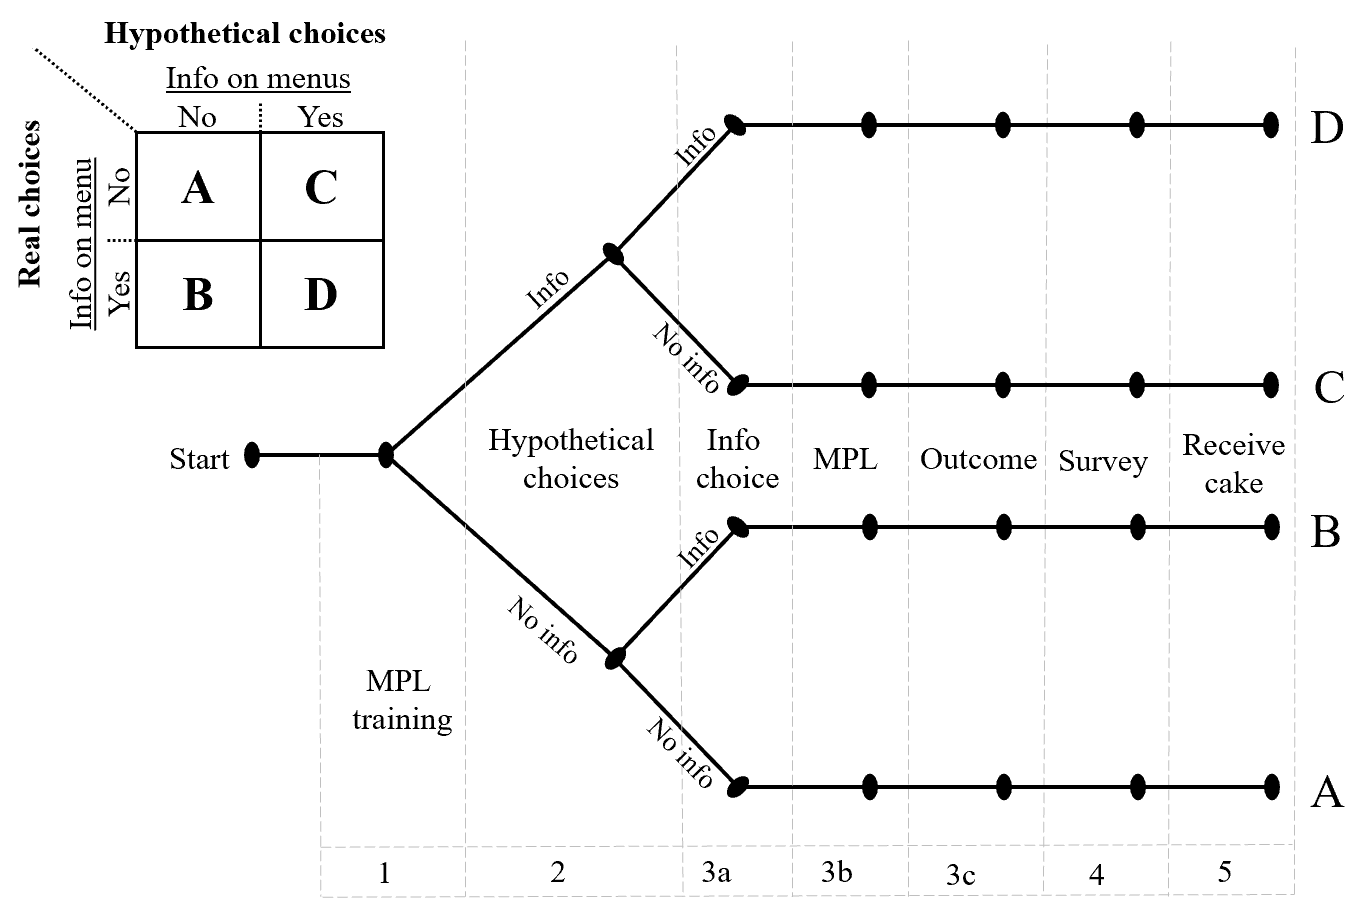
\includegraphics[width=1\textwidth]{./figures/experimentalDesign.png}}
  \end{center}
\end{figure}

Based on our recruitment flyer, all participants knew they would receive a cake for their participation in the experiment. After that, the experiment followed the structure shown in Figure \ref{fig:expDesign}. In step (1), we taught participants how to use a multiple-price list (MPL) and evaluated their understanding. In step (2), we asked participants to choose their preferred dessert from eleven consecutive dessert menus, each showing three desserts. These choices were not incentivized, and we were explicit about their hypothetical nature. In this step, we randomized half of the participants to see menus without calorie information and the other half to see menus with calorie information. The goal of this manipulation was to exercise some control over potential heterogeneity in expectations about information that participants might have brought to the laboratory. Making a series of choices from menus \emph{without} calorie information should set a baseline of \emph{low} expectations of receiving information when moving to the experiment’s next step, and making a series of choices from menus \emph{with} calorie information should set a baseline of \emph{high} expectations of receiving information.

In step (3a) participants were once again shown a menu with three new desserts. One of these, a cake, was marked as the dessert they were about to actually receive, to eat after the experiment.\footnote{We marked the cake they would receive for two reasons. First, we were not able to offer participants their dessert choice from a menu. As a compromise, to keep the menu structure used earlier, we marked the cake they would receive. Second, and more importantly, we wanted participants to focus on the choice of calorie information instead of the choice of dessert.} Within each baseline group established in step (2), we again randomized participants into two groups, resulting in a $2 \times 2$ design. One group was \emph{more endowed} with calorie information about the desserts, in the sense that the menu already showed a calorie-information column. However, the actual calorie numbers were \enquote{temporarily} \emph{xxx}-ed out, and participants in this group were asked whether they wanted to \enquote{keep} the calorie information, so they would see it, or \enquote{remove} the calorie information. The exact wording used is shown in Figure \ref{fig:expManipulation} (top panel). The other group was \emph{less endowed} with calorie information, in the sense that the menu showed nothing calorie-related to begin with. Participants in this group were asked whether they wanted to \enquote{add} calorie information, so they would see it, or \enquote{keep} calorie information \enquote{off}. The exact wording used is shown in Figure  \ref{fig:expManipulation} (bottom panel).

\begin{figure}[ht]
  \caption{Key experimental manipulation}\label{fig:expManipulation}
  \begin{center}
  {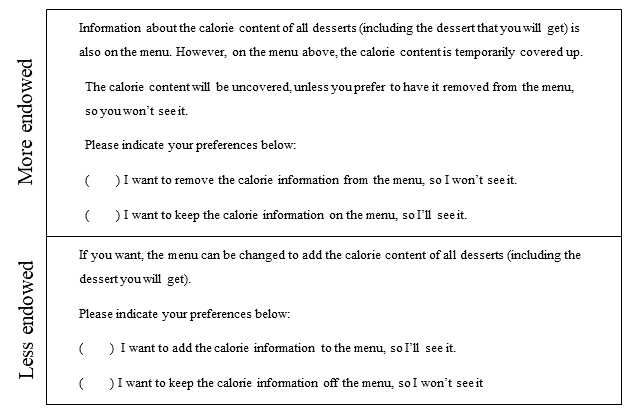
\includegraphics[width=1\textwidth]{./figures/keyManipulation.png}}
  \end{center}
\end{figure}

We argue that, compared to participants in the \emph{less endowed} treatment, participants in the \emph{more endowed} treatment were more likely to expect to receive calorie information about their cake, for three reasons. First, the presence of \emph{xxx}-ed out calorie-information column on the menu was intended to make \emph{more endowed} participants focus first on getting calorie information when considering whether they want to actually see it, whereas the absence of any such information for \emph{less endowed} participants was intended to make them focus first on not getting it. Second, the menu description pointed to the calorie information as already being on the menu for \emph{more endowed} participants, but as needing a change in the menu for \emph{less endowed} participants. And third, the description of how participants could choose to see the information used \enquote{I want to keep} for \emph{more endowed} participants, but \enquote{I want to add} for \emph{less endowed} participants.

% check usage of MPL

In step (3b) we aimed to elicit a monetary value for calorie information, using a multiple-price list that allowed this value to range from negative to positive. For example, if participants chose to see the calorie information in step (3a), thereby indicating that information had positive value for them, we gave them the option to either keep the information on the menu (i.e., stick with their initial choice and ultimately see the information) or remove the information and receive some additional money. That is, we elicited their Willingness To Accept (WTA) to \emph{not} see the information after all. Conversely, if participants chose not to see the information in step (3a), thereby indicating that information had negative value for them, we elicited their WTA to \emph{see} the information after all, in a similar fashion.

The multiple-price list included 10 choices, with monetary amounts ranging from \$0.01 to \$5.00.\footnote{The complete list of values in the MPL is \$0.01, \$0.25, \$0.50, \$0.75, \$1.00, \$1.50, \$2.00, \$2.50, \$3.00, and \$5.00.}  Once all 10 choices were made, one choice was randomly selected to be binding.

In step (3c), participants were shown a menu on which the calorie information of the cake they were about to receive was either revealed or not, depending on the outcome of the multiple-price list. In step (4), participants answered survey questions about their demographics, attitudes (risk preferences, time preferences, and degree of self-control), health status, health concern (the importance they assigned to their own health), and familiarity with calorie information (see Appendix \ref{appendix:background} for a description of these data). Finally, in step (5), participants received their payment (show-up fee plus earnings from the MPL) and cake.

\subsection{Identification strategy}

Based on our two consecutive manipulations to influence participants’ expectations about receiving calorie information, we organize participants in four groups: A, B, C, and D (see Figure \ref{fig:expDesign}). In the first manipulation, participants in groups A and B chose desserts from menus without calorie information, whereas participants in groups C and D chose desserts from menus with calorie information. In the second manipulation, participants in groups A and C chose whether to add information to a menu, whereas participants in groups B and D chose whether to keep information on a menu.

Because we are manipulating expectations, the timing and order of the manipulations matter. Specifically, for participants induced by the first manipulation to have high baseline expectations of receiving information (groups C and D), we expect the effect size of the second manipulation to be smaller. We therefore analyze that effect size separately for each baseline (i.e., groups A and B separately from groups C and D).

For each baseline, we identify the endowment effect by relating our experimental design to our theoretical definition of an endowment effect in equation \ref{eq:endowmentEffect}: $U(L^i|R^i)-U(L^u|R^i)>U(L^i|R^u)-U(L^u|R^u)$. For example, for participants induced by the first manipulation to have low baseline expectations of receiving information (groups A and B), being \emph{more endowed} with information in the second manipulation corresponds to having reference lottery $R^i$ (group B, left-hand side of the equation), while being \emph{less endowed} corresponds to having reference lottery $R^u$ (group A, right-hand side of the equation). Within each group, choosing to receive information corresponds to choosing outcome lottery $L^i$, while choosing not to receive information corresponds to choosing outcome lottery $R^u$. Thus, we can infer whether $U(L^i|R^i)-U(L^u|R^i)$ is positive ($L^i$ is chosen) or negative for each participant in group B, and similarly infer whether $U(L^i|R^u)-U(L^u|R^u)$ is positive or negative for each participant in group A. Then, we aggregate the choices of each group and simply compare the share of participants in group A who chose to receive information to the share of participants in group B who did so.\footnote{However, we note that our experimental results are contingent on the unverified manipulation of expectations (i.e., probabilistic beliefs). First, we assume that making eleven choices using menus with or without calorie information changes the probabilistic belief to expect to receive information. Second, given the probabilistic belief previously assumed to have been manipulated, we assume that presenting a menu with or without covered calorie information, along with other framing differences, would further change the probability belief to expect to receive information or not. We chose not to verify that the manipulations in fact had the intended effect in forming the expectation to receive information. One alternative would have been to ask participants whether they were expecting to receive information after each manipulation, however, we thought that such verification would have unintendedly changed the expectations. A second alternative would have been to use a different experimental design to manipulate the expectations. Following \citet{marzilliericsonExpectationsEndowmentsEvidence2011} \citet{heffetzEndowmentEffectExpectations2014}, one could manipulate the expectations, for example to expect to receive information, by telling participants that they have a 1\% chance to be able to choose whether to get the information or not, and a 99\% chance to receive the information (more recently, \citet{cerulli-harmsRandomizingEndowmentsExperimental2019} show that forced exchange is preferred than the allowable exchange used by \citet{marzilliericsonExpectationsEndowmentsEvidence2011} and \citet{heffetzEndowmentEffectExpectations2014}). The advantage of this approach is that one can verify that participants formed the correct expectations with a quiz evaluating the understanding of the statement. However, we think that our approach is more appropriate for the context of information and closer to potential policy applications outside of the laboratory. Overall, as reflected by the sensitivity of results to changes in the experimental environment documented in the empirical literature of expectations-based reference-dependent models, we can only conclude that manipulating expectations is a challenging task in which trade-offs are inevitable.} Furthermore, the heterogeneity in the data can be rationalized by assuming random utility.\footnote{Explicitly, participants could be heterogeneous (for example) in terms of self-control, curiosity, or concern about calorie intake.}

Our main goal is to show that preferences for information are not standard, and to propose that these preferences are reference-dependent. Therefore, we use the model of standard preferences as a straw man to set up null hypotheses to be rejected \citet{dellavignaChapterStructuralBehavioral2018}. Explicitly, we test the null hypothesis that the share of participants who choose to receive information is the same regardless of endowment status against the alternative that the share is higher for \emph{more endowed} participants. Note that the distinction between the DA approach and the KR approach does not play any role in the experiment: our design does not set out to distinguish between the two.\footnote{\citet{sprengerEndowmentEffectRisk2015} tests for the existence of an endowment effect for monetary risk using a design that does purposely distinguish between the DA and the KR approach. He shows that the data supports the KR approach instead of the DA approach.}

\subsection{Results}


We find evidence supporting the existence of an endowment effect for information: more participants chose to receive information when they were \emph{more endowed} with it (i.e., when getting a menu with temporarily \emph{xxx}-ed out calorie information). Furthermore, as expected, the effect was smaller for participants first primed to expect to receive information (i.e., participants who made initial hypothetical choices from menus with calorie information). A discussion of the empirical analysis and the results follows.

\subsubsection{Estimation strategy}

The practical goal of the analysis is to estimate the causal effect of receiving a menu with \emph{xxx}-ed out calorie information ($R^i$), relative to receiving a menu without \emph{xxx}-ed out calorie information ($R^u$), on the choice of receiving information ($L^i$) or not ($L^u$). Because we rely on the randomization process as identification strategy, unbiasedness of the unconditional ordinary least squares (OLS) estimator of the average treatment effect is guaranteed both under large- and finite-sample assumptions. However, the unbiasedness property guarantees only that the true treatment effect can be recovered by averaging the treatment effect over all potential realizations.\footnote{In general, the definition of a realization depends on the sources of uncertainty accounted for in the analysis. If only design-based uncertainty is considered, a realization is one draw of all possible randomizations within the population. If only sampling-based uncertainty is considered, a realization is one sample drawn from a superpopulation. Finally, if both sources of uncertainty are considered, a realization is a particular randomization from a particular sample \citep{abadieSamplingBasedDesignBasedUncertainty2020}.} In practice, however, we get only one estimate of the treatment effect, obtained from the one realization we observe. This observed estimate reflects, in addition to the true treatment effect, any imbalances between treatment groups of variables that are prognostic (i.e., correlated with the dependent variable). For example, if by chance one treatment group ends up with 70\% rather than 50\% of the female participants, and if being female is prognostic, then the estimate of the treatment effect will be influenced by the gender imbalance.

Given that our sample size for estimating the treatment effect of the key experimental manipulation is about 110 participants, the estimate is likely to reflect covariate imbalances. Consequently, to address the uncertainty regarding the extent to which these imbalances matter, we present estimates from both the unconditional OLS estimator and from all possible conditional OLS estimators that can be created by adjusting the regression with all combinations of the set of prognostic covariates with large imbalances between groups.\footnote{There are no objective criteria to define \emph{large}. The term is subjective and roughly means \enquote{large enough to affect the treatment effect in an economically significant way.} We describe the method used to identify the set of covariates with large imbalances between treatment groups in Appendix \ref{appendix:largeImbalances}.} Under large-sample assumptions, both the unconditional and the conditional estimators are unbiased. However, because the correlation between a covariate and the treatment variable might be different from zero, the conditional estimators present in our analyses are biased under finite-sample assumptions.\footnote{There are at least two alternatives to avoid the trade-off between unbiasedness and adjustments for covariate imbalance.

Ex-ante, one can use a randomized block design to force balance in prognostic covariates \citet{atheyChapterEconometricsRandomized2017}. However, this design requires a solid understanding of the covariates that are prognostic of information preferences, as well as baseline data with those prognostic covariates. For this study, it was not feasible to use a randomized block design, because we did not have the baseline data and we were not willing to compromise the incentivized choices in the experiment by asking survey questions up front.

Ex-post, if one can create binary covariates\textemdash from the original covariates\textemdash and they partition the population, the OLS estimator of the average treatment effect is unbiased when a full set of interactions is included \citep{linAgnosticNotesRegression2013,atheyChapterEconometricsRandomized2017}. This approach is not feasible for our study either because, even if we could create binary covariates that partition the population, we do not have enough observations to estimate the regression with a full set of interactions.
}

\subsubsection{Results using choice data}

We first present the results for participants not primed with calorie information (low baseline, groups A and B). The share of these participants who chose to receive information was $71\%$ for those \emph{more endowed} with information vs. $52\%$ for those \emph{less endowed} ($p=0.02$ from a $t$-test and $p=0.05$ from a Fisher’s exact test,  both one-sided).\footnote{We use Simon Heß’s Stata program ritest \citep{hessRandomizationInferenceStata2017} with 5000 random permutations and the coefficient of the treatment from an OLS regression as the test statistic for our Fisher’s exact tests \citet{imbensCausalInferenceStatistics2015}.} Figure \ref{fig:resultsLowBaseline} shows the implied treatment effect of $0.19$ and its associated $p$-value from an unconditional OLS regression, as well as 255 estimates and associated $p$-values from all possible adjusted regressions that can be estimated using the eight covariates with large imbalances between treatment groups A and B.

\begin{figure}[ht]
  \caption{Estimates of the treatment effect for participants in the \emph{low} baseline \\ (using choice data)}\label{fig:resultsLowBaseline}
  \begin{center}
  {\includegraphics[width=1\textwidth]{./figures/hypotheticalChoices_noInfo.png}}
  \end{center}
\end{figure}

Of these 256 point-estimates, 100\% are higher than $0.10$, 96.5\% are higher than $0.15$, and 20.1\% are higher than $0.20$. In addition, 99.6\%, 82\%, and 0\% of the estimates are statistically significant at the standard $0.1$, $0.05$, and $0.01$ levels of significance. Overall, we interpret these results as strong evidence for the existence of an endowment effect for information.

Next, we present the results for participants primed with calorie information (high baseline, groups C and D). The share of these participants who chose to receive information was 65.5\% for those \emph{more endowed} with information vs. 59.5\% for those \emph{less endowed} ($p=0.27$ from a $t$-test and $p=0.34$ from a Fisher’s exact test, both one-sided). Figure \ref{fig:resultsHighBaseline} shows the implied treatment effect of $0.06$ and its associated $p$-value from an unconditional OLS regression, as well as 512 estimates and associated $p$-values from all possible adjusted regressions that can be estimated using the nine covariates with large imbalances between treatment groups C and D.

\begin{figure}[ht]
  \caption{Estimates of the treatment effect for participants in the \emph{high} baseline \\ (using choice data)}\label{fig:resultsHighBaseline}
  \begin{center}
  {\includegraphics[width=1\textwidth]{./figures/hypotheticalChoices_info.png}}
  \end{center}
\end{figure}

Of these 512 point-estimates, 100\% are higher than $0$, 99.8\% are higher than $0.05$, 86\% are higher than $0.10$, 19\% are higher than $0.15$, and none are higher than $0.20$. In addition, 63\%, 10.5\%, and 0\% of the estimates are statistically significant at the standard $0.1$, $0.05$, and $0.01$ levels of significance. Overall, we interpret these results also as support for existence of an endowment effect\textemdash only one of the 512 point estimates is smaller than $0.05$. However, the size of the endowment effect is smaller for the primed participants of groups C and D than for the unprimed participants of groups A and B.

\subsubsection{Results using WTA data}

Finally, we designed the experiment to gather Willingness-To-Accept (WTA) data (from the multiple-price list) as an alternative measure of preferences for information. That is, we planned to reproduce the analyses presented above using, instead of the binary choice whether to receive information as a discrete dependent variable, WTA as a continuous dependent variable. Ex post, however, we realized that our way of eliciting WTA may not keep the relevant reference lottery constant, which makes it a questionable measure of participants’ value of information. For example, a participant randomized to receive a menu with \emph{xxx}-ed out calorie information (the \emph{more endowed} treatment) starts out with reference lottery $R^i$ and then chooses to either have the information revealed, corresponding to outcome lottery $L^i$, or taken off the menu, corresponding to outcome lottery $L^u$. From her choice, we obtain our binary measure of information preferences by inferring that $U(L^i|R^i)-U(L^u|R^i)$ is positive if $L^i$ is chosen, and negative if $L^u$ is chosen. If she chooses to receive information, we elicit her WTA to take the information off the menu after all. This WTA is plausibly a measure of the weakly positive utility $U(L^i|R^i)-U(L^u|R^i)$ that she forgoes by giving up information. If, however, she chooses to take the information off, we elicit her WTA to keep the information on after all, and have it be revealed. At that point, we lose control of her referent. Although the WTA measures the weakly positive utility $U(L^u|\cdot)-U(L^i|\cdot)$, it is unclear whether she still considers herself endowed with information, which would imply that her reference lottery when completing the multiple-price list is still $R^i$, or whether her initial choice to take the endowed information off the menu changes her reference lottery to $R^u$.

This lack of clarity reflects a broader gap in our understanding of the referent formation process. \citet{koszegiModelReferenceDependentPreferences2006} simply assume that the reference point depends on expectations held \enquote{in the recent past}, rather than expectations held at the time of consumption. They add that
\begin{displayquote}
  This does not assume that beliefs are slow to adjust to new information \emph{or that people are unaware of the choices that they have just made}\textemdash but that preferences do not instantaneously change when beliefs do. When somebody finds out five minutes ahead of time that she will for sure not receive a long-expected \$100, she would presumably immediately adjust her expectations to the new situation, but she will still five minutes later assess not getting the money as a loss. (p.1141, emphasis added).
\end{displayquote}

Applied to our context, this assumption implies that a participant’s choice of a particular outcome lottery need not instantaneously change her reference lottery. That is, she may still, at least for a while, feel endowed with information even if she just chose to give it up, or feel not endowed with information even if she just chose to get it.\footnote{Experimental results reported by \citet{heffetzAreReferencePoints2018} in fact suggest that reference points do not necessarily change to match beliefs even gradually, through the mere passage of time.  Instead, \enquote{some sense of internalization of, or getting used to, the new expectations} is required (p.5).}

Nevertheless, we cannot \emph{rule out} that a participant's choice to either receive or not receive information might have moved her referent before completing the multiple-price list. As a result, we cannot treat the difference in information values elicited through our multiple-price list for \emph{more endowed} and \emph{less endowed} participants as an estimate of the endowment effect expressed in dollar terms. What we can say is that, if an endowment effect does in fact exist, then any movement of participants' referents with their choices will bias downwards the elicited difference in information valuations.

The reason is straightforward. Let $\Re^i$ denote the subset of \emph{more endowed} participants, and $\Re^u$ the subset of \emph{less endowed} participants. If participants' choice did \emph{not} move their referents, then the endowment effect could be estimated as the average revealed value of information for \emph{more endowed} participants minus the average revealed value of information for \emph{less endowed} participants:
\begin{equation*}
  \frac{\sum_{j \in \Re^i}[U_j(L_j^i|R_j^i)-U_j(L_j^u|R_j^i)]}
       {|\Re^i|}
  -
  \frac{\sum_{j \in \Re^u}[U_j(L_j^i|R_j^u)-U_j(L_j^u|R_j^u)]}
      {|\Re^u|}.
\end{equation*}

If, on the other hand, participants' choices did move their referents, then the first average would be \enquote{contaminated} by some terms $U_j(L_j^i|R_j^u)-U_j(L_j^u|R_j^u)$, and the second average by some terms $U_j(L_j^i|R_j^i)-U_j(L_j^u|R_j^i)$. Suppose now that an endowment effect in fact exists (as defined in Equation \ref{eq:endowmentEffect}). Any contamination of the kind described will then tend to \emph{lower} the first average, since the contaminated terms $U_j(L_j^i|R_j^u)-U_j(L_j^u|R_j^u)$ will tend to be lower than the terms $U_j(L_j^i|R_j^i)-U_j(L_j^u|R_j^i)$ that they replace in the summation. Conversely, contamination will tend to \emph{raise} the second average, since the contaminated terms $U_j(L_j^i|R_j^i)-U_j(L_j^u|R_j^i)$ will tend to be higher than the terms $U_j(L_j^i|R_j^u)-U_j(L_j^u|R_j^u)$ that they replace. The upshot is that contamination will tend to reduce the estimated endowment effect relative to its true value.

Despite our potentially \emph{contaminated} estimates of the value of information, we still find that our results using WTA data are consistent with the existence of an endowment effect for information. We present the results for participants in the low and the high baseline below.\footnote{We follow \citet{allcottWelfareEffectsNudges2019} to calculate the value of the information for each participant from the choices in the multiple-price list. That is, we use the mean of the start and end points for the interior intervals and assume the conditional distribution of the WTA to be triangular for the open intervals. The results are robust to alternative assumptions (see the online supplementary material).}

For participants not primed with calorie information (low baseline, groups A and B), the average value of the information for those \emph{more endowed} was \$0.55 vs. \$0.08 for those \emph{less endowed} ($p=0.11$ from a $t$-test and $p=0.11$ from a Fisher's exact test, both one-sided). Figure \ref{fig:resultsLowBaselineWTA} shows the implied treatment effect of $0.46$ and its associated $p$-value from an unconditional OLS regression, as well as 256 estimates and associated $p$-values from all possible adjusted regressions that can be estimated using the eight covariates with large imbalances between groups A and B.

Of these 256 point-estimates, 100\% are higher than $\$0.2$, 94.15\% are higher than $\$0.25$, and 34.4\% are higher than $\$0.5$. In addition, 25.4\%, 6.64\%, and 0\%, of the estimates are statistically significant at the standard $0.1$, $0.05$, and $0.01$ levels of significance. Overall, we interpret also these results as support for the existence of the endowment effect\textemdash all 256 point-estimates are higher than $\$0.2$.

% ADD A NOTE OR FOOTNOTE ABOUT WHY RESULTS ARE WEAKER. CONTAMINATION AND LESS POWER TO DETECT EFFECT ARE TWO OF THEM. ????????????????????????????????

\begin{figure}[ht]
  \caption{Estimates of the treatment effect for participants in the \emph{low} baseline \\ (using WTA data)}\label{fig:resultsLowBaselineWTA}
  \begin{center}
  {\includegraphics[width=1\textwidth]{./figures/hypotheticalChoices_NoInfoWTA.png}}
  \end{center}
\end{figure}

For participants primed with calorie information (high baseline, groups C and D). The average value of the information for those \emph{more endowed} was \$0.56 vs. \$0.29 for those \emph{less endowed} ($p=0.24$ from a $t$-test and $p=0.21$ from a Fisher's exact test, both one-sided). Figure \ref{fig:resultsHighBaselineWTA} shows the implied treatment effect of $\$0.26$ and its associated $p$-value from an unconditional OLS regression, as well as 512 estimates and associated $p$-values from all possible adjusted regressions that can be estimated using the eight covariates with large imbalances between groups C and D.

Of these 512 point-estimates, 100\% are higher than $\$0.2$, 96.6\% are higher than $\$0.25$, and 0\% are higher than $\$0.5$. In addition, 15.6\%, 0\%, and 0\%, of the estimates are statistically significant at the standard $0.1$, $0.05$, and $0.01$ levels of significance. Overall, we interpret also these results as support for the existence of the endowment effect\textemdash all point-estimates are higher than $\$0.2$.

\begin{figure}[ht]
  \caption{Estimates of the treatment effect for participants in the \emph{high} baseline \\ (using WTA data)}\label{fig:resultsHighBaselineWTA}
  \begin{center}
  {\includegraphics[width=1\textwidth]{./figures/hypotheticalChoices_InfoWTA.png}}
  \end{center}
\end{figure}


\section{Results}

  
We find evidence supporting the existence of an endowment effect for information: more participants chose to receive information when they were endowed with it (i.e., when getting a menu with temporarily \emph{xxx}-ed out calorie information). Furthermore, as expected, the effect was smaller for participants first primed to expect to receive information (i.e., participants who made initial hypothetical choices from menus with calorie information). A discussion of the empirical analysis and the results follows.

\subsection{Estimation strategy}

The practical goal of the analysis is to estimate the causal effect of receiving a menu with \emph{xxx}-ed out calorie information ($R^i$), relative to receiving a menu without \emph{xxx}-ed out calorie information ($R^u$), on the choice of receiving information ($L^i$) or not ($L^u$). Because we rely on the randomization process as identification strategy, unbiasedness of the unconditional ordinary least squares (OLS) estimator of the average treatment effect is guaranteed both under large- and finite-sample assumptions. However, the unbiasedness property guarantees only that the true treatment effect can be recovered by averaging the treatment effect over all potential realizations.\footnote{In general, the definition of a realization depends on the sources of uncertainty accounted for in the analysis. If only design-based uncertainty is considered, a realization is one draw of all possible randomizations within the population. If only sampling-based uncertainty is considered, a realization is one sample drawn from a superpopulation. Finally, if both sources of uncertainty are considered, a realization is a particular randomization from a particular sample \citet{abadieSamplingBasedDesignBasedUncertainty2020}.} In practice, however, we get only one estimate of the treatment effect, obtained from the one realization we observe. This observed estimate reflects, in addition to the true treatment effect, any imbalances between treatment groups of variables that are prognostic (i.e., correlated with the dependent variable). For example, if by chance one treatment group ends up with 70\% rather than 50\% of the female participants, and if being female is prognostic, then the estimate of the treatment effect will be influenced by the gender imbalance.

Given that our sample size for estimating the treatment effect of the key experimental manipulation is about 110 participants, the estimate is likely to reflect covariate imbalances. Consequently, to address the uncertainty regarding the extent to which these imbalances matter, we present estimates from both the unconditional OLS estimator and from all possible conditional OLS estimators that can be created by adjusting the regression with all combinations of the set of prognostic covariates with large imbalances between groups.\footnote{There are no objective criteria to define \emph{large}. The term is subjective and roughly means \enquote{large enough to affect the treatment effect in an economically significant way.} We describe the method used to identify the set of covariates with large imbalances between treatment groups in Appendix \ref{appendix:largeImbalances}.} Under large-sample assumptions, both the unconditional and the conditional estimators are unbiased. However, because the correlation between a covariate and the treatment variable might be different from zero, the conditional estimators present in our analyses are biased under finite-sample assumptions.\footnote{There are at least two alternatives to avoid the trade-off between unbiasedness and adjustments for covariate imbalance.

Ex-ante, one can use a randomized block design to force balance in prognostic covariates \citet{atheyChapterEconometricsRandomized2017}. However, this design requires a solid understanding of the covariates that are prognostic of information preferences, as well as baseline data with those prognostic covariates. For this study, it was not feasible to use a randomized block design, because we did not have the baseline data and we were not willing to compromise the incentivized choices in the experiment by asking survey questions up front.

Ex-post, if one can create binary covariates\textemdash from the original covariates\textemdash and they partition the population, the OLS estimator of the average treatment effect is unbiased when a full set of interactions is included \citep{linAgnosticNotesRegression2013,atheyChapterEconometricsRandomized2017}. This approach is not feasible for our study either because, even if we could create binary covariates that partition the population, we do not have enough observations to estimate the regression with a full set of interactions.
}

\subsection{Results using choice data}

We first present the results for participants not primed with calorie information (low baseline, groups A and B). The share of these participants who chose to receive information was $71\%$ for those endowed with information vs. $52\%$ for those not endowed ($p=0.02$ from a $t$-test and $p=0.05$ from a Fisher’s exact test,  both one-sided).\footnote{We use Simon Heß’s Stata program ritest \citep{hessRandomizationInferenceStata2017} with 5000 random permutations and the coefficient of the treatment from an OLS regression as the test statistic for our Fisher’s exact tests \citet{imbensCausalInferenceStatistics2015}.} Figure \ref{fig:resultsLowBaseline} shows the implied treatment effect of $0.19$ and its associated $p$-value from an unconditional OLS regression, as well as 255 estimates and associated $p$-values from all possible adjusted regressions that can be estimated using the eight covariates with large imbalances between treatment groups A and B.

\begin{figure}[ht]
  \caption{Estimates of the treatment effect for participants in the \emph{low} baseline \\ (using choice data)}\label{fig:resultsLowBaseline}
  \begin{center}
  {\includegraphics[width=1\textwidth]{./figures/hypotheticalChoices_noInfo.png}}
  \end{center}
\end{figure}

Of these 256 point-estimates, 100\% are higher than $0.10$, 96.5\% are higher than $0.15$, and 20.1\% are higher than $0.20$. In addition, 99.6\%, 82\%, and 0\% of the estimates are statistically significant at the standard $0.1$, $0.05$, and $0.01$ levels of significance. Overall, we interpret these results as strong evidence for the existence of an endowment effect for information.

Next, we present the results for participants primed with calorie information (high baseline, groups C and D). The share of these participants who chose to receive information was 65.5\% for those endowed with information vs. 59.5\% for those not endowed ($p=0.27$ from a $t$-test and $p=0.34$ from a Fisher’s exact test, both one-sided). Figure \ref{fig:resultsHighBaseline} shows the implied treatment effect of $0.06$ and its associated $p$-value from an unconditional OLS regression, as well as 512 estimates and associated $p$-values from all possible adjusted regressions that can be estimated using the nine covariates with large imbalances between treatment groups C and D.

\begin{figure}[ht]
  \caption{Estimates of the treatment effect for participants in the \emph{high} baseline \\ (using choice data)}\label{fig:resultsHighBaseline}
  \begin{center}
  {\includegraphics[width=1\textwidth]{./figures/hypotheticalChoices_info.png}}
  \end{center}
\end{figure}

Of these 512 point-estimates, 100\% are higher than $0$, 99.8\% are higher than $0.05$, 86\% are higher than $0.10$, 19\% are higher than $0.15$, and none are higher than $0.20$. In addition, 63\%, 10.5\%, and 0\% of the estimates are statistically significant at the standard $0.1$, $0.05$, and $0.01$ levels of significance. Overall, we interpret these results also as support for existence of an endowment effect\textemdash only one of the 512 point estimates is smaller than $0.05$. However, the size of the endowment effect is smaller for the primed participants of groups C and D than for the unprimed participants of groups A and B.

\subsection{Results using WTA data}

Finally, we designed the experiment to gather Willingness-To-Accept (WTA) data (from the multiple-price list) as an alternative measure of preferences for information. That is, we planned to reproduce the analyses presented above using, instead of the binary choice whether to receive information as a discrete dependent variable, WTA as a continuous dependent variable. Ex post, however, we realized that our way of eliciting WTA may not keep the relevant reference lottery constant, which makes it a questionable measure of participants’ value of information. For example, a participant randomized to receive a menu with \emph{xxx}-ed out calorie information (the \emph{endowed} treatment) starts out with reference lottery $R^i$ and then chooses to either have the information revealed, corresponding to outcome lottery $L^i$, or taken off the menu, corresponding to outcome lottery $L^u$. From her choice, we obtain our binary measure of information preferences by inferring that $U(L^i|R^i)-U(L^u|R^i)$ is positive if $L^i$ is chosen, and negative if $L^u$ is chosen. If she chooses to receive information, we elicit her WTA to take the information off the menu after all. This WTA is plausibly a measure of the weakly positive utility $U(L^i|R^i)-U(L^u|R^i)$ that she forgoes by giving up information. If, however, she chooses to take the information off, we elicit her WTA to keep the information on after all, and have it be revealed. At that point, we lose control of her referent. Although the WTA measures the weakly positive utility $U(L^u|\cdot)-U(L^i|\cdot)$, it is unclear whether she still considers herself endowed with information, which would imply that her reference lottery when completing the multiple-price list is still $R^i$, or whether her initial choice to take the endowed information off the menu changes her reference lottery to $R^u$.

This lack of clarity reflects a broader gap in our understanding of the referent formation process. \citet{koszegiModelReferenceDependentPreferences2006} simply assume that the reference point depends on expectations held \enquote{in the recent past}, rather than expectations held at the time of consumption. They add that
\begin{displayquote}
  This does not assume that beliefs are slow to adjust to new information \emph{or that people are unaware of the choices that they have just made}\textemdash but that preferences do not instantaneously change when beliefs do. When somebody finds out five minutes ahead of time that she will for sure not receive a long-expected \$100, she would presumably immediately adjust her expectations to the new situation, but she will still five minutes later assess not getting the money as a loss. (p.1141, emphasis added).
\end{displayquote}

Applied to our context, this assumption implies that a participant’s choice of a particular outcome lottery need not instantaneously change her reference lottery. That is, she may still, at least for a while, feel endowed with information even if she just chose to give it up, or feel not endowed with information even if she just chose to get it.\footnote{Experimental results reported by \citet{heffetzAreReferencePoints2018} in fact suggest that reference points do not necessarily change to match beliefs even gradually, through the mere passage of time.  Instead, \enquote{some sense of internalization of, or getting used to, the new expectations} is required (p.5).}

Nevertheless, we cannot \emph{rule out} that a participant's choice to either receive or not receive information might have moved her referent before completing the multiple-price list. As a result, we cannot treat the difference in information values elicited through our multiple-price list for endowed and not endowed participants as an estimate of the endowment effect expressed in dollar terms. What we can say is that, if an endowment effect does in fact exist, then any movement of participants' referents with their choices will bias downwards the elicited difference in information valuations.

The reason is straightforward. Let $\Re^i$ denote the subset of endowed participants, and $\Re^u$ the subset of not endowed participants. If participants' choice did \emph{not} move their referents, then the endowment effect could be estimated as the average revealed value of information for endowed participants minus the average revealed value of information for not endowed participants:
\begin{equation*}
  \frac{\sum_{j \in \Re^i}[U_j(L_j^i|R_j^i)-U_j(L_j^u|R_j^i)]}
       {|\Re^i|}
  -
  \frac{\sum_{j \in \Re^u}[U_j(L_j^i|R_j^u)-U_j(L_j^u|R_j^u)]}
      {|\Re^u|}.
\end{equation*}

If, on the other hand, participants' choices did move their referents, then the first average would be \enquote{contaminated} by some terms $U_j(L_j^i|R_j^u)-U_j(L_j^u|R_j^u)$, and the second average by some terms $U_j(L_j^i|R_j^i)-U_j(L_j^u|R_j^i)$. Suppose now that an endowment effect in fact exists (as defined in Equation \ref{eq:endowmentEffect}). Any contamination of the kind described will then tend to \emph{lower} the first average, since the contaminated terms $U_j(L_j^i|R_j^u)-U_j(L_j^u|R_j^u)$ will tend to be lower than the terms $U_j(L_j^i|R_j^i)-U_j(L_j^u|R_j^i)$ that they replace in the summation. Conversely, contamination will tend to \emph{raise} the second average, since the contaminated terms $U_j(L_j^i|R_j^i)-U_j(L_j^u|R_j^i)$ will tend to be higher than the terms $U_j(L_j^i|R_j^u)-U_j(L_j^u|R_j^u)$ that they replace. The upshot is that contamination will tend to reduce the estimated endowment effect relative to its true value.

Despite our potentially \emph{contaminated} estimates of the value of information, we still find that our results using WTA data are consistent with the existence of an endowment effect for information. We present the results for participants in the low and the high baseline below.\footnote{We follow \citet{allcottWelfareEffectsNudges2019} to calculate the value of the information for each participant from the choices in the multiple-price list. That is, we use the mean of the start and end points for the interior intervals and assume the conditional distribution of the WTA to be triangular for the open intervals. The results are robust to alternative assumptions (see the online supplementary material).}

For participants not primed with calorie information (low baseline, groups A and B), the average value of the information for those endowed was \$0.55 vs. \$0.08 for those not endowed ($p=0.11$ from a $t$-test and $p=0.11$ from a Fisher's exact test, both one-sided). Figure \ref{fig:resultsLowBaselineWTA} shows the implied treatment effect of $0.46$ and its associated $p$-value from an unconditional OLS regression, as well as 256 estimates and associated $p$-values from all possible adjusted regressions that can be estimated using the eight covariates with large imbalances between groups A and B.

Of these 256 point-estimates, 100\% are higher than $\$0.2$, 94.15\% are higher than $\$0.25$, and 34.4\% are higher than $\$0.5$. In addition, 25.4\%, 6.64\%, and 0\%, of the estimates are statistically significant at the standard $0.1$, $0.05$, and $0.01$ levels of significance. Overall, we interpret also these results as support for the existence of the endowment effect\textemdash all 256 point-estimates are higher than $\$0.2$.

% ADD A NOTE OR FOOTNOTE ABOUT WHY RESULTS ARE WEAKER. CONTAMINATION AND LESS POWER TO DETECT EFFECT ARE TWO OF THEM. ????????????????????????????????

\begin{figure}[ht]
  \caption{Estimates of the treatment effect for participants in the \emph{low} baseline \\ (using WTA data)}\label{fig:resultsLowBaselineWTA}
  \begin{center}
  {\includegraphics[width=1\textwidth]{./figures/hypotheticalChoices_NoInfoWTA.png}}
  \end{center}
\end{figure}

For participants primed with calorie information (high baseline, groups C and D). The average value of the information for those endowed was \$0.56 vs. \$0.29 for those not endowed ($p=0.24.X$ from a $t$-test and $p=0.21$ from a Fisher's exact test, both one-sided). Figure \ref{fig:resultsHighBaselineWTA} shows the implied treatment effect of $\$0.26$ and its associated $p$-value from an unconditional OLS regression, as well as 512 estimates and associated $p$-values from all possible adjusted regressions that can be estimated using the eight covariates with large imbalances between groups C and D.

Of these 512 point-estimates, 100\% are higher than $\$0.2$, 96.6\% are higher than $\$0.25$, and 0\% are higher than $\$0.5$. In addition, 15.6\%, 0\%, and 0\%, of the estimates are statistically significant at the standard $0.1$, $0.05$, and $0.01$ levels of significance. Overall, we interpret also these results as support for the existence of the endowment effect\textemdash all point-estimates are higher than $\$0.2$.

\begin{figure}[ht]
  \caption{Estimates of the treatment effect for participants in the \emph{high} baseline \\ (using WTA data)}\label{fig:resultsHighBaselineWTA}
  \begin{center}
  {\includegraphics[width=1\textwidth]{./figures/hypotheticalChoices_InfoWTA.png}}
  \end{center}
\end{figure}


\section{Conclusion}

  % SUMMARY

The general topic of this paper is how people value information; and the key insight is that information preferences are reference-dependent. The ex-ante value assigned to a particular piece of information depends on, at least, one prior belief (i.e., the referent) about the delivery (do I expect to get it?), content (do I expect bad news?), or usefulness (do I expect to change anything in response?) of that piece of information. Further, due to the incorporeal nature of information, all possible referents are expectations-based. In this paper we focus on the case in which the referent is a prior belief about the delivery of information.

More precisely, in this paper we predict and find evidence for an \enquote{endowment effect for information}, which is a tendency to value information more if getting the information is expected than if it is not expected. The two leading theories of expectations-based reference-dependent preferences---the Disappointment Aversion and the Kőszegi and Rabin approach---imply this effect when information is instrumental, but only the Kőszegi and Rabin approach predicts this effect when information is not instrumental. Further, we find evidence supporting the prediction of an endowment effect for information in a laboratory experiment that manipulates participants’ expectations to receive instrumental information.

% CBA implications

The existence of this endowment effect for information complicates welfare analysis because the effect implies that net benefits of information policies may vary with people’s expectations. In other words, consumers who regularly see information about the calories in their food, the risks of drunk driving, or the benefits of exercising may come to expect access to such information and then end up valuing it more.\footnote{For example, to gain support for an information policy, politicians may therefore choose to first implement the policy as a trial with a clear end date, with the intent to reevaluate the policy at that point (the public might be more willing to accept a trial of a policy). Such increase in public support after a trial period has been found for other policies---\citet{cherryImpactTrialRuns2014} show that public acceptance of a congestion tax increased after a trial period with the tax.} As such, the existence of an endowment effect for information implies that the role of the referent, including potential heterogeneity of referents across consumers, ought to be explicitly acknowledged and accounted for in welfare analysis.

On the other hand, the same implication that the net benefits of information policies may vary with people’s expectations points towards a potential new policy tool to reduce the tendency to avoid \enquote{good} information (e.g., information about health risk). Beyond policies to provide information, the new policy tool would focus on raising people’s expectation to receive information. In turn, via the endowment effect, this expectation would increase people’s valuation of information (which leads to less information avoidance).\footnote{As this new policy tool aims to manipulate expectations, the process by which people form expectations would need to be better understood. \possessivecitet{heffetzAreReferencePoints2018} refinement of \possessivecitet{koszegiModelReferenceDependentPreferences2006} definition of the referent is a step in the right direction (i.e., the referent is lagged beliefs that have \enquote{sunk-in}, instead of just lagged beliefs). Future research may explore whether referent spill-overs across domains of information occur: does having information in one domain increase people’s expectations of getting information in general?}


\clearpage



% REFERENCES -------------------------------------------------------------------

\bibliography{endowmentEffectInfo}

\clearpage


% APPENDICES -------------------------------------------------------------------
\begin{appendices}

  \startcontents[sections]
  \printcontents[sections]{l}{1}{\setcounter{tocdepth}{1}}

  \clearpage

\section{Proofs and derivations}

    \label{appendix:theory}

    \begin{center}
\textbf{Non-instrumental information}
\end{center}

Under the DA approach, applying the general formula
\begin{equation*}
  U(L|R) \equiv \sum_{n=1}^N p_n\biggl\{u(x_n) + \mu\biggl(u(x_n) - \sum_{m=1}^M q_m
u(r_m)\biggr)\biggr\}
\end{equation*}
yields that
\begin{align*}
  U(L^i|R^i)
&= p_1\bigl\{x_1 + \mu\bigl(x_1 - \underbrace{[q_1r_1 + q_2r_2]}_{E[R^i]}\bigr)\bigr\}
 + p_2\bigl\{x_2 + \mu\bigl(x_2 - \underbrace{[q_1r_1 + q_2r_2]}_{E[R^i]}\bigr)\bigr\}
\\
&= \half\bigl\{h + \bigl(h - [\half h + \half\ell]\bigr)\bigr\}
 + \half\bigl\{\ell + \lambda\bigl(\ell - [\half h + \half \ell]\bigr)\bigr\}
\\
&= [\half h + \half \ell] + \half\bigl(h - [\half h + \half\ell]\bigr)
   - \half\lambda\bigl([\half h + \half \ell] - \ell\bigr)
\\
&= [\half h + \half \ell] - \qrtr(\lambda - 1)(h - \ell).
\end{align*}
If the person ends up getting information, then with probability $\half$ she
will learn that the cake is low-calorie. She will then get high intrinsic
utility $h$ from consuming it, and will in addition experience \enquote{elation} $h - [\half h + \half\ell] > 0$, because $h$ exceeds the intrinsic utility $\half h + \half \ell$ that she expected to get---her reference utility. Also with probability $\half$, however, the cake will turn out to be high-calorie. The person will then get low intrinsic utility $\ell$ from consuming it, and will in addition experience \enquote{disappointment} $\lambda(\ell - [\half h + \half\ell]) < 0$, because $\ell$ falls short of her reference utility. If $\lambda > 1$, the disappointment will outweigh the elation, leaving her with expected intrinsic utility $\half h + \half \ell$ from consuming the cake, but in addition net negative expected gain-loss utility $- \qrtr(\lambda - 1)(h - \ell) < 0$.

The same formula yields that
\begin{align*}
  U(L^u|R^i)
&= p\bigl\{x + \mu\bigl(x - \underbrace{[q_1r_1 + q_2r_2]}_{E[R^i]}\bigr)\bigr\}
\\
&= 1\cdot\bigl\{[\half h + \half \ell] + \bigl([\half h + \half \ell] - [\half h + \half \ell]\bigr)\bigr\}\\
&= [\half h + \half \ell].
\end{align*}
Here, because the person ends up not getting information, she will get average
intrinsic utility $\half h + \half \ell$ for sure. And because this is exactly
what she expected to get, she experiences no elation or disappointment.

Comparing the two utilities yields that
\begin{equation*}
  U(L^i|R^i) - U(L^u|R^i) = -\qrtr(\lambda-1)(h-\ell) < 0.
\end{equation*}
This shows that, because the person is disappointment averse ($\lambda > 1$),
she will also be information adverse: she perceives herself as better off
staying ignorant, because her disappointment from getting bad news would
outweigh her elation from getting good news.

Crucially, this result holds regardless of whether she started out expecting
to get information or not, i.e., with reference lottery $R^i$ or $R^u$. This
follows because the DA approach \enquote{collapses} the reference lottery into its expectation before evaluating gain-loss utility. Since $R^i$ and $R^u$
have the same expectation $E[R^i] = E[R^u] = q_1r_1 + q_2r_2$, it follows that
$U(L^i|R^u) = U(L^i|R^i)$ and $U(L^u|R^u) = U(L^u|R^i)$, so also
\begin{equation*}
  U(L^i|R^u) - U(L^u|R^u) = U(L^i|R^i) - U(L^u|R^i) = -\qrtr(\lambda-1)(h-\ell) < 0.
\end{equation*}
There is, in other words no endowment effect for information: the person is
equally information adverse, regardless of whether she expects to get
information or not.

Under the KR approach, however, the situation is quite different. Applying the
general formula
\begin{equation*}
  U(L|R) \equiv \sum_{n=1}^N p_n\biggl\{u(x_n) + \sum_{m=1}^M q_m
\mu\bigl(u(x_n) - u(r_m)\bigr)\biggr\}
\end{equation*}
yields that
\begin{align*}
  U(L^i|R^i)
&= p_1\bigl\{x_1 + q_1\mu(x_1 - r_1) + q_2\mu(x_1 - r_2)\bigr\}
 + p_2\bigl\{x_2 + q_1\mu(x_2 - r_1) + q_2\mu(x_2 - r_2)\bigr\}\\
&= \half\bigl\{h + \half(h - h) + \half\underbrace{(h - \ell)}_{\text{gain}}\bigr\}
 + \half\bigl\{\ell + \half\underbrace{\lambda(\ell - h)}_{\text{loss}} + \half(\ell - \ell)\bigr\}\\
&= [\half h + \half \ell] +
    \qrtr (h-\ell) - \qrtr \lambda(h-\ell)\\
&= [\half h + \half \ell] - \qrtr(\lambda-1)(h - \ell).
\end{align*}
If the person ends up getting information, she will learn with
probability $\half$ that the cake is low-calorie and then get high intrinsic
utility $h$ from consuming it. In addition (differently from the DA approach), she will compare that utility {\em separately} to the two outcomes $h$ or $\ell$ that she expected to possibly get. Since she started out expecting to get $h$ with probability $\half$, she will experience no elation from that first
comparison; but since she expected to get only $\ell$ with probability $\half$
also, she will experience gain-utility $h-\ell>0$ from that second comparison. With complementary probability $\half$, she will learn that the cake is high-calorie, and then get low intrinsic utility $\ell$ from consuming it. In addition, when comparing that utility separately to the
two outcomes $h$ or $\ell$ that she expected to possibly get, she will experience loss-utility $\lambda(\ell - h) < 0$ from the first comparison, and no gain-loss utility from the second comparison. Aggregating over all these
permutations leaves her with expected intrinsic utility $\half h + \half \ell$
from consuming the cake, but in addition net negative expected gain-loss
utility $-\qrtr(\lambda - 1)(h - \ell) < 0$.

The same formula yields that
\begin{align*}
  U(L^u|R^i)
&= p\bigl\{x + q_1\mu(x - r_1) + q_2\mu(x - r_2)\bigr\}
\\
&= 1\cdot\bigl\{[\half h + \half \ell] + \half\underbrace{\lambda([\half h + \half \ell] - h)}_{\text{loss}} + \half\underbrace{([\half h + \half \ell] - \ell)}_{\text{gain}}\bigr\}\\
&= [\half h + \half \ell] +
   \half\left([\half h + \half \ell] - \ell\right)
   -\half\lambda\left(h - [\half h + \half \ell]\right)\\
&= [\half h + \half \ell] - \qrtr(\lambda-1)(h - \ell).
\end{align*}
Because the person ends up not getting information, she will get
average intrinsic utility $\half h + \half \ell$ for sure. In addition, when comparing that utility separately to the two outcomes $h$ or $\ell$ she expected to possibly get, she will experience loss utility $\lambda([\half h + \half \ell] - h) < 0$ from the first comparison, and gain utility $[\half h + \half\ell] - \ell$ from the second comparison. Aggregating leaves her with expected intrinsic utility $\half h + \half \ell$ from consuming the cake, but in addition net negative expected gain-loss utility $-\qrtr(\lambda - 1)(h -
\ell) < 0$.

Comparing these first two utilities yields that
\begin{equation*}
  U(L^i|R^i) - U(L^u|R^i) = 0.
\end{equation*}
This shows that, despite being disappointment averse, the person is indifferent
to getting information or not. The reason becomes clear if we rewrite $U(L^i|R^i)$ and $U(L^u|R^i)$ as follows:
\begin{align*}
  U(L^i|R^i) &= [\half h + \half \ell] +
  \qrtr \underbrace{(h-\ell)}_{\text{gain}} +
  \qrtr \underbrace{\lambda(\ell-h)}_{\text{loss}}\\
  U(L^u|R^i) &= [\half h + \half \ell] +
  \half\underbrace{\left([\half h + \half \ell] - \ell\right)}_{\text{gain}} +
  \half\underbrace{\lambda\left([\half h + \half \ell]-h\right)}_{\text{loss}}.
\end{align*}
Relative to becoming informed, staying ignorant cuts both the gain and loss
utilities in half (from $[\half h + \half \ell] - \ell$ to $h - \ell$, and
from $-\lambda(h - [\half h + \half \ell])$ to $-\lambda(h - \ell)$,
respectively). But because it simultaneously doubles the probability that
either the gain utility or the loss utility will be experienced (from $\half$
to $\qrtr$), the net effect is a wash.

Next, we have
\begin{align*}
  U(L^i|R^u)
&= p_1\bigl\{x_1 + q\mu(x_1 - r)\bigr\}
 + p_2\bigl\{x_2 + q\mu(x_2 - r)\bigr\}\\=
&= \half\bigl\{h +
 1\cdot\underbrace{(h - [\half h + \half\ell])}_{\text{gain}}\bigr\}
 + \half\bigl\{\ell + 1\cdot\underbrace{\lambda(\ell - [\half h + \half\ell])}_{\text{loss}}\bigr\}\\
&= [\half h + \half \ell] +
\half(h-[\half h + \half \ell]) - \half \lambda([\half h + \half\ell] - \ell)\\
&= [\half h + \half \ell] - \qrtr(\lambda-1)(h - \ell).
\end{align*}
If the person did not expect to be informed but ends up getting information,
she will compare the intrinsic utility from the outcomes $h$ and $\ell$ to the
utility $\half h + \half \ell$ that she expected to get. The gain-utility $h -
[\half h + \half \ell]>0$ with probability $\half$ will again be outweighed by
the loss-utility $ - \half \lambda([\half h + \half\ell] - \ell)<0$ with
probability $\half$, resulting in net negative expected gain-loss utility
$-\qrtr(\lambda - 1)(h - \ell) < 0$.

Lastly, we have
\begin{align*}
  U(L^u|R^u)
&= p\bigl\{x + q\mu(x - r)\bigr\}
\\
&= 1\cdot\bigl\{[\half h + \half \ell] + 1\cdot([\half h + \half \ell] - [\half
h + \half \ell])\bigr\}\\
&= [\half h + \half \ell].
\end{align*}
Since the person gets exactly what she expects, namely no information for
sure, she experiences no gain-loss utility.

Comparing the second two utilities yields that
\begin{equation*}
  U(L^i|R^u) - U(L^u|R^u) = -\qrtr(\lambda-1)(h-\ell) < 0.
\end{equation*}
This shows that, if the person expects not to get information, she will be
information adverse. Moreover, since we found above that
\begin{equation*}
  U(L^i|R^i) - U(L^u|R^i) = 0,
\end{equation*}
i.e., that the person is indifferent about information if she {\em does} expect
to get it, we now do have an endowment effect for information: the value of
information is higher, namely zero instead of negative, for people who expect
to get it.

\begin{center}
\textbf{Instrumental information}
\end{center}

Up until this point, we have treated information as non-instrumental, i.e., as not used by the person to adjust her behavior in any way. What if the person does make adjustments if she learns the actual calorie content of the cake, for example eating more or less of it, or changing her exercise routine later that day?

Suppose for simplicity that these adjustments increase the person's utility by the same amount $\Delta>0$, and define $h^* \equiv h+\Delta$ and $\ell^* \equiv \ell + \Delta$. Ex ante, she should then expect to get intrinsic utility $\half h^* + \half \ell^*$ if she ends up learning the cake's calorie content, but only $\half h + \half \ell$ if she does not.

As a result, assuming adjustments are not so large as to make $[\half h + \half \ell]-\ell^*$ negative, which requires that $\Delta<\half (h-\ell)$, the four different utilities under the KR approach change as follows:
\begin{align*}
  U(L^i|R^i)
    &= \half \bigl\{h^* + \half (h^*-h^*) + \half (h^* - \ell^*)\bigr\} +
       \half \bigl\{\ell^* + \half \lambda (\ell^*-h^*) + \half (\ell^*-\ell^*)\bigr\}
    \\
    &= [\half h^* + \half \ell^*] - \qrtr (\lambda - 1)(h^*-\ell^*)
    \\
    &= [\half h + \half \ell] + \Delta - \qrtr (\lambda-1)(h-\ell)
    \\
  U(L^u|R^i)
    &= [\half h + \half \ell] + \half ([\half h + \half \ell] - \ell^*) -
    \half \lambda (h^*-[\half h + \half \ell])
    \\
    &= [\half h + \half \ell] - \qrtr (\lambda - 1)(h-\ell)-
    \half(\lambda+1)\Delta
    \\
  U(L^i|R^u)
    &= [\half h^* + \half \ell^*] + \half (h^* - [\half h + \half \ell]) -
    \half \lambda ([\half h + \half \ell] - \ell^*)
    \\
    &= [\half h + \half \ell] + \Delta - \qrtr(\lambda-1)(h-\ell)+
    \half (\lambda + 1)\Delta
    \\
  U(L^i|R^u)
    &= [\half h + \half \ell].
\end{align*}

Comparing the first two utilities yields
\begin{equation*}
  U(L^i|R^i) - U(L^u|R^i) = \Delta + \half (\lambda+1)\Delta.
\end{equation*}
While previously the person was indifferent about getting information if she started out expecting to get it, she now strictly prefers getting information, because of the use she can make of it.

Comparing the second two utilities yields
\begin{equation*}
  U(L^i|R^u) - U(L^u|R^u) = - \qrtr (\lambda-1)(h-\ell) + \half (\lambda + 3) \Delta.
\end{equation*}
Whereas previously the person was information averse if she started out expecting to remain ignorant, she may now prefer getting information that is sufficiently useful. Nevertheless, the overall gain from information is still higher if she starts out expecting to get it than if she does not, so that an endowment effect for information continues to exist.

Under the DA approach, we now get
\begin{align*}
  U(L^i|R^i)
    &= \half \bigl\{h^* + (h^* - [\half h^* + \half \ell^*])\bigr\} +
       \half \bigl\{\ell^* + \lambda(\ell^* - [\half h^* + \half \ell^*]) \bigr\}
    \\
    &= [\half h^* + \half \ell^*] - \qrtr (\lambda - 1)(h^*-\ell^*)
    \\
    &= [\half h + \half \ell] + \Delta - \qrtr (\lambda-1)(h-\ell)
    \\
  U(L^u|R^i)
    &= 1\cdot \bigl\{ [\half h + \half \ell] + \lambda([\half h + \half \ell] - [\half h^* + \half \ell^*]) \bigr\}
    \\
    &= [\half h + \half \ell] - \lambda \Delta
    \\
  U(L^i|R^u)
    &= \half \bigl\{h^* + (h^* - [\half h + \half \ell])\bigr\} +
       \half \bigl\{\ell^* + \lambda(\ell^* - [\half h + \half \ell]) \bigr\}
    \\
    &= [\half h^* + \half \ell^*] - \qrtr (\lambda - 1)(h^* - \ell^*) +
       \half (\lambda + 1)\Delta
    \\
    &= [\half h + \half \ell] + \Delta - \qrtr (\lambda-1)(h-\ell) +
       \half (\lambda + 1)\Delta
    \\
  U(L^i|R^u)
    &= 1\cdot \bigl\{ [\half h + \half \ell] + ([\half h + \half \ell]-[\half h + \half \ell]) \bigr\}
    \\
    &= [\half h + \half \ell].
\end{align*}
Comparing the first and second utilities yields
\begin{align*}
  U(L^i|R^i) - U(L^u|R^i)
    &= -\qrtr (\lambda-1)(h-\ell) + (\lambda + 1) \Delta
    \\
  U(L^i|R^u) - U(L^u|R^u)
    &= -\qrtr (\lambda-1)(h-\ell) + \half (\lambda + 3) \Delta.
\end{align*}
Whereas previously the person was information averse regardless of whether she expected to get information or not, she may now be information loving, provided the information is sufficiently useful. Moreover, because $\lambda>1$ implies that $\lambda + 1 > \half (\lambda+3)$, we now have an endowment effect for information under the DA approach as well.

Close examination of the four utility expressions reveals why. If the person starts out expecting to be informed, and therefore expecting to get $\half h^* + \half \ell^*$, the unexpectedly \emph{not} getting information results in a loss of intrinsic utility $\Delta$ for sure, with associated loss utility $\lambda \Delta$ for sure. The overall gain in utility from getting information is therefore $\Delta + \lambda \Delta = (\lambda+1)\Delta$. If the person starts out expecting to stay ignorant, however, then unexpectedly getting information results in a gain of intrinsic utility $\Delta$ for sure. If the news is good, however, with probability $\half$, then the gain comes as a pleasant surprise, gives her additional gain utility $\Delta$; but if the news are bad, also with probability $half$, then the gain merely mitigates an unpleasant surprise, reducing her loss utility by $\lambda \Delta$. The overall gain in utility from getting information is therefore only $\Delta + [\half \Delta + \half \lambda \Delta]=\half(\lambda+3)\Delta$.


    % add link back to document

    \clearpage

\section{Participants and procedures}

    \label{appendix:participants}

    % \documentclass[12pt]{article}
%
% \usepackage[utf8]{inputenc}
% \usepackage[english]{babel}
% \usepackage{indentfirst}
%
% \begin{document}

We recruited 267 participants during the Spring of 2018, most of them from the University of Wyoming. After excluding 1 student with dietary restrictions (e.g., vegan or lactose intolerance), 18 students who participated in a different experiment with the same researchers a few weeks before this experiment, and 29 students who reported they did not intend to eat the cake themselves (implying that calorie content would not matter to them), we ended up with 219 valid observations.

We completed the experiment in 13 sessions with about 20 participants each; all of them with the same monitor in the same experimental laboratory of the College of Business in the University of Wyoming.\footnote{Aiming to \emph{normalize} the hunger level of participants during the experiment, we conducted all sessions either before lunch (11 AM) or before dinner (5 PM)} Upon arrival to the laboratory, we assigned participants to one of the computers and asked them not to communicate with each other or use their cell phones during the experiment. The session started with a short lecture with examples on how to use a multiple-price list.\footnote{The slides used for the lecture are included in the online supplementary material} After that, each participant started the experiment on their own. The experiment, including randomizations, were done using Qualtrics. At the end of the experiment, we paid each participant in a private room. They received a \$20 show-up fee plus \$1.46 on average for their earnings in the multiple-price list. Finally, we gave each participant one dessert that we bought from a major supermarket.\footnote{We covered the information about the calorie content in the nutritional label with a marker before the experiment started.} On average, the experiment took about 35 minutes.

% \end{document}


    % add link back to document

    \clearpage

\section{Background data}

    \label{appendix:background}

    \begin{table}[h] \centering
\newcolumntype{C}{>{\centering\arraybackslash}X}

\caption{Descriptive statistics}
\label{tab:descriptiveStatistics}
\begin{tabularx}{\linewidth}{lCCCCC}

\toprule
{}&{N}&{Mean}&{Std. Dev.}&{Min.}&{Max.} \tabularnewline
\midrule \addlinespace[\belowrulesep]
Female&219&.46&.5&0&1 \tabularnewline
Age&219&21.79&4.44&18&46 \tabularnewline
College&219&.92&.27&0&1 \tabularnewline
Expenses level&211&.65&.4&.2&2.1 \tabularnewline
Income level&201&9.94&9.47&5&60 \tabularnewline
Body-Mass Index&219&24.3&5.08&.25&47.59 \tabularnewline
Underweight&219&.05&.23&0&1 \tabularnewline
normalWeight&219&.74&.44&0&1 \tabularnewline
Overweight&219&.18&.38&0&1 \tabularnewline
Obese&219&.01&.12&0&1 \tabularnewline
\midrule Risk preferences&219&3.45&1.29&1&6 \tabularnewline
Food self-control&219&29.05&6.31&13&50 \tabularnewline
Present-bias (\(\beta\))&213&.93&1.22&.03&17.5 \tabularnewline
Discount factor (\(\delta\))&213&.87&.22&.02&1 \tabularnewline
Hunger level&219&1.56&.83&0&3 \tabularnewline
\midrule Health assessment&219&3.62&.86&1&5 \tabularnewline
Would benefit from eating healthier&219&4.32&.59&2&5 \tabularnewline
Wish could eat healthier at home&219&3.54&1.03&1&5 \tabularnewline
Wish could eat healthier out&219&3.44&1.04&1&5 \tabularnewline
Importance of eating healthy food&219&3.48&.87&1&5 \tabularnewline
Importance of exercising regularly&219&3.98&1.02&1&5 \tabularnewline
Importance of healthy body weight&219&4.18&.88&1&5 \tabularnewline
\midrule Knows calorie needs&219&3.82&.59&2&6 \tabularnewline
Experience with calorie information&219&2.94&1.06&1&5 \tabularnewline
Frequency visits to chain restaurants&219&3.35&1.01&1&6 \tabularnewline
\bottomrule 

\end{tabularx}
\end{table}



    % add link back to document

    \clearpage

\section{Identifying large covariate imbalances between groups}

    \label{appendix:largeImbalances}

    % \documentclass[12pt]{article}
%
% \usepackage[utf8]{inputenc}
% \usepackage[english]{babel}
% \usepackage{csquotes}
% \usepackage{mathtools}
% \usepackage{hyperref}
% \usepackage{geometry}
% \usepackage{amsfonts}
% \usepackage{amsmath}
% \usepackage{amssymb}
% \usepackage{graphicx}
% \usepackage[small,bf,center]{caption}
% \usepackage{subfig}
% \usepackage{setspace}
% \usepackage{float}
% \usepackage[section]{placeins} % for \FloatBarrier
% \usepackage{indentfirst}
% \usepackage[toc,page]{appendix}
%
% \usepackage{natbib}
%   \bibliographystyle{chicago}
%
%
% \begin{document}

\subsection{Method}

In this section we describe the method used to identify prognostic covariates with \emph{large} imbalances between groups. We started with 22 potential covariates from the answers to the survey questions at the end of the experiment.\footnote{We do not claim to have captured \emph{all} the characteristics that may be prognostic of information preferences, instead, we used our expertise to identify the ones we considered to be more important. As with any other empirical study, the rest will be captured in the error term of the econometric analyses.} We chose not to try to subjectively assess the degree of prognosis of each of these variables, instead, we assumed that all of these variables are prognostic of the dependent variable\textemdash i.e., information preferences. Thus, the task was only to identify \emph{large} imbalances between groups.

We used an eclectic approach to identify \emph{large} differences, but our method closely follows advice given by \citet{imbensCausalInferenceStatistics2015} to assess differences in the distribution of a covariates between groups in the context of observational studies. For each covariate in each pair of groups, we calculated the univariate normalized difference in means, the multivariate difference in covariate distributions, and the natural logarithm of the ration of standard deviations. A description of each estimator, taken from \citet{imbensCausalInferenceStatistics2015} follows.

% CHECK BOOK FOR PAGE AND ACCURACY

\begin{displayquote}

Let $\bar{X_c}$ and $\bar{X_t}$ denote the sample averages of the covariate values for the control and treatment group respectively:

\begin{equation*}
  \bar{X_c}=\frac{1}{N_c} \sum_{i:W_i=0} X_i
  \text{  and  }
  \bar{X_t}=\frac{1}{N_t} \sum_{i:W_i=0} X_i,
\end{equation*}

where (\ldots) $N_c$ is the number of control units, and $N_t$ is the number of treated units. Also, let $s_c^2$ and $s_t^2$ denote the conditional within-group sample variances of the covariate:

\begin{equation*}
  s_c^2=\frac{1}{N_c-1} \sum_{i:W_i=0} (X_i-\bar{X_c})^2
  \text{  and  }
  s_t^2=\frac{1}{N_t-1} \sum_{i:W_i=0} (X_i-\bar{X_t})^2,
\end{equation*}

\end{displayquote}

Then the estimator of the normalized difference of means is

\begin{equation*}
  \hat{\Delta}_{ct}=
    \frac{\bar{X_t}-\bar{X_c}}
         {\sqrt{\frac{s_c^2+s_c^2}{2}}}
\end{equation*}

% CHECK REFERENCES BELOW

As a rule of thumb, \citet{imbensCausalInferenceStatistics2015} say \enquote{\ldots when treatment groups have important covariates that are more than one-quarter or one-half of a standard deviation apart, simple regression methods are unreliable for removing biases associated with differences in covariates\ldots} (p.277).\footnote{First, we note that this rule of thumb is given in the context of observational studies. Second, we note that there are at least three versions of the normalized differences in means estimator in work by Guido Imbens and they all share the same rule of thumb (i.e., differences larger than 0.25 standard deviations are large). We use the version in \citet{imbensCausalInferenceStatistics2015} because it is the most recent. In Imbens \& Woolridge (2009, pp 24, JEL), the estimator sums up the variances but does not divide by 2. In Imbens \& Woolridge (NBER summer, 2007, p.34) and Imbens \& Wooldrige (Cemmep, UCL, 2000), the denominator is only the sum of the variances. Because different estimators share the same rule of thumb (although the last version does include two thresholds) along with the fact that we have not found the supporting evidence behind the rule of thumb, we take the rule of thumb as expert advice but do not rely solely on this rule to conclude.} \citet{imbensCausalInferenceStatistics2015} also suggest to use the multivariate difference in covariate distributions (p.313), however, there is no clear guidance on how large a difference should be to be considered \emph{large}.\footnote{In their illustrations on chapter 14, \citet{imbensCausalInferenceStatistics2015} interpret some of the multivariate difference in distribution estimates. In page 320, they interpret an estimate of 1.78 as suggestive that \enquote{…overall the two groups are substantially apart}. In page 353, a table including an estimate of 1.49 is discussed and interpreted as evidence of substantial differences, but the multivariate differences in distribution estimator is not interpreted directly. In page 324, a table including an estimate of 0.44 is discussed and interpreted as \enquote{suggesting that the balance in covariates is excellent\ldots}, but it does not interpret the estimator directly. Following this interpretation, one could consider differences lower or equal than 0.44 as small and differences higher or equal to 1.49 as large.}

We also compared measures of dispersion of the covariates between groups. Using the same notation from \citet{imbensCausalInferenceStatistics2015} described above, the estimator is the natural logarithm ratio of standard deviations
\begin{equation*}
  \hat{\Gamma}_{ct}=ln(s_t)-ln(s_c).
\end{equation*}
We did not find any practical guidance to assess whether a difference is large or not.

These measures\textemdash univariate and multivariate difference in means and logarithm ratio of standard deviations\textemdash give us a way to compare distributions based on the first two moments of their distributions. However, we found that insufficient to capture imbalances that would matter if a covariate is prognostic. Instead of inspecting normalized differences for higher-order moments of the distributions, as suggested in page 313 by \citet{imbensCausalInferenceStatistics2015}, we take their complementary advice:

\begin{displayquote}
  Finally, it may be useful to construct histograms of the distribution of a covariate in both treatment arms to detect visually subtle differences not captured by differences in means and variances, especially for covariates that are a priori believed to be highly associated with the outcomes.
\end{displayquote}

Consequently, for each variable, we used the results of the comparison of the normalized differences of means and variances, and the visual inspection of the histograms (or kernel densities for continuous variables), to subjectively identify \emph{large} differences.

\subsection{Results}

Here, we summarize the covariates with \emph{large} imbalances between groups identified for each of the three pairs of groups. In the online supplementary material, we include a detailed description of the application of the method for each pair of groups.

First, we compare the group of participants who received menus without calorie information in their hypothetical choices (low baseline, groups A and B) to the group of participants who received menus with calorie information in their hypothetical choices (high baseline, groups C and D). There is only one covariate with a \emph{large} imbalance: riskPref (higher in no info).

% ADD TABLE

Second, within participants who received a menu without calorie information for their hypothetical choices (low baseline, groups A and B), we compare the group of people who received a menu without covered calorie information for their real choice (group A) to the group of people who received a menu with covered calorie information for their real choice (group B).

There are 8 covariates with \emph{large} imbalances. Of them, 4 are higher in the no info group (expCat,  riskPref, beta, prevExp) and 4 are higher in the info group (collegeDegree, healthStatus, wishEatBetterOut, calNeedsKnowledge).

Third, within participants who received a menu with calorie information for their hypothetical choices (groups C and D), we compare the group of people who received a menu without covered calorie information for their real choice (group C) to the group of people who received a menu with covered calorie information for their real choice (group D).

There are 10 covariates with \emph{large} imbalances. Of them, 3 are higher in the no info group (exerciseImportant, weightImportant, calNeedsKnowledge), 5 are higher in the info group (age, collegeDegree, hungry, healthStatus, chain), and 2 are unclear (expCat, prevExp).

% \end{document}


    % add link back to document

    \clearpage

\section{Description of online supplementary material}

  \label{appendix:onlineSupplementaryMaterial}

  The following supplementary material is available online (\textbf{XXXXX}):

\begin{itemize}
  \item Questionnaire

  \item Data cleaning

  \item Identification of \emph{large} differences in covariates between groups

  \item Robustness to alternative WTA assumptions

  \item MPL training slides  
\end{itemize}


\end{appendices}


\end{document}

% END OF FILE ------------------------------------------------------------------
% ------------------------------------------------------------------------------
